%%%%%%%%%%%%%%%%%%%%%%%%%%%%%%%%%%%%%%%%%%%%%%%%%%%%%%%%%%
%
% eXascale Infolab thesis template -- Bachelor and Masters
% version 1.1, Oct 2019
%
%%%%%%%%%%%%%%%%%%%%%%%%%%%%%%%%%%%%%%%%%%%%%%%%%%%%%%%%%%
%
% Based on:
% Masters/Doctoral Thesis
% LaTeX Template Version 2.5 (27/8/17)
% http://www.LaTeXTemplates.com
% CC BY-NC-SA 3.0 (http://creativecommons.org/licenses/by-nc-sa/3.0/)
%
%%%%%%%%%%%%%%%%%%%%%%%%%%%%%%%%%%%%%%%%%

\documentclass[11pt,english,singlespacing,headsepline,consistentlayout]{structure/XI_thesis}

%----------------------------------------------------------------------------------------
%	LATEX PACKAGES
%----------------------------------------------------------------------------------------

%%%%%%%%%%%%%%%%%%%%%%%%%%% DO NOT EDIT
\usepackage[utf8]{inputenc} % Required for inputting international characters
\usepackage[T1]{fontenc} % Output font encoding for international characters
\usepackage{mathpazo} % Use the Palatino font by default
\usepackage[backend=bibtex,style=authoryear,natbib=true]{biblatex} % Use the bibtex backend with the authoryear citation style
\usepackage[autostyle=true]{csquotes} % Required to generate language-dependent quotes in the bibliography
\usepackage{booktabs}       % professional-quality tables
\usepackage{array}          % custom sizes for table columns
\usepackage{amssymb}        % extended blackboard math symbols
\usepackage{amsmath}        % complete AMS math package
% \usepackage[english]{babel} % spelling / syllabification
\usepackage{algorithm}      % pseudocode float
\usepackage[noend]{algpseudocode}  % pseudocode macros
\usepackage{graphicx}       % include graphics
\usepackage{epstopdf}       % vectorial graphics
\usepackage{subcaption}     % sub captions
\usepackage{url}            % URLs
%%%%%%%%%%%%%%%%%%%%%%%%%%% DO NOT EDIT - end

% Define path and extensions for your graphics
\graphicspath{{figures/}}%{{../jpeg/} [...]}
\DeclareGraphicsExtensions{.pdf,.jpg,.jpeg,.png,eps}


%% User packages
% \usepackage{add here}
% Include your package settings in `structure/settings.tex`


% Load package settings
% !TEX root = ../main.tex

%----------------------------------------------------------------------------------------
% PACKAGE CONFIGURATIONS
%----------------------------------------------------------------------------------------

% Filename of the bibliography
\addbibresource{structure/main.bib}

% Margin settings
\geometry{
  paper=a4paper, % Paper format
  inner=2.5cm, % Inner margin
  outer=3.8cm, % Outer margin
  bindingoffset=.5cm, % Binding offset
  top=1.5cm, % Top margin
  bottom=1.5cm, % Bottom margin
  %showframe, % Uncomment to show how the type block is set on the page
}

% Figures location
\graphicspath{{figures/}}
\DeclareGraphicsExtensions{.pdf,.png,.jpg,.jpeg,.eps,.ps}

% Todo notes
\usepackage[backgroundcolor=pink]{todonotes}
% algorithms
\usepackage{algorithm}
\usepackage[noend]{algpseudocode}
% plots
\usepackage{pgfplots}
\pgfplotsset{compat = newest}
% visualization in mutliple rows
\usepackage{enumitem}
\newenvironment{figrow}%
{%
\centering\addtocounter{figure}{1}% if caption at bottom
\begin{enumerate}[%
itemsep=2pt,parsep=0em,
label={(\alph*)},
ref={\thefigure.(\alph*)}
]}%
{\end{enumerate}\addtocounter{figure}{-1}}
% for python code
\usepackage{minted}
% Code listings, with syntax highlighting
\usepackage{listings}

% Load custom thesis information (remember to fill in)
% !TEX root = ../main.tex

%----------------------------------------------------------------------------------------
% THESIS INFORMATION
%----------------------------------------------------------------------------------------

\thesistitle{Alternative Models for Direct Policy Search in Reinforcement Learning Control Problems} % Your thesis title, this is used in the title and abstract, print it elsewhere with \ttitle
\supervisor{Dr. Giuseppe Cuccu} % Your supervisor's name, this is used in the title page, print it elsewhere with \supname
\cosupervisor{Prof. Dr. Philippe Cudré-Mauroux} % If you have a co-supervisor, include it here. This is used in the title page, print it elsewhere with \supname
\degree{Master} % Your degree name, this is used in the title page and abstract, print it elsewhere with \degreename
\author{Corina Masanti} % Your name, this is used in the title page and abstract, print it elsewhere with \authorname
\addresses{Bd de Pérolles 90} % Your address, this is not currently used anywhere in the template, print it elsewhere with \addressname

\subject{Computer Science} % Your subject area, this is not currently used anywhere in the template, print it elsewhere with \subjectname
\keywords{black-box optimization, reinforcement learning, binary trees, neural networks, random weight guessing, polynomials} % Keywords for your thesis, this is not currently used anywhere in the template, print it elsewhere with \keywordnames
\university{\href{http://www.unifr.ch}{University of Fribourg}} % Your university's name and URL, this is used in the title page and abstract, print it elsewhere with \univname
\department{\href{https://www3.unifr.ch/inf/fr/}{Department of Informatics}} % Your department's name and URL, this is used in the title page and abstract, print it elsewhere with \deptname
\group{\href{https://www3.unifr.ch/inf/en/exascale-infolab.html}{eXascale Infolab}} % Your research group's name and URL, this is used in the title page, print it elsewhere with \groupname
\faculty{\href{https://www3.unifr.ch/scimed/fr/}{Faculty of Science and Medicine}} % Your faculty's name and URL, this is used in the title page and abstract, print it elsewhere with \facname

% Set title, author and keywords on the compiled PDF
\AtBeginDocument{
  \hypersetup{pdftitle=\ttitle} % Set the PDF's title to your title
  \hypersetup{pdfauthor=\authorname} % Set the PDF's author to your name
  \hypersetup{pdfkeywords=\keywordnames} % Set the PDF's keywords to your keywords
}

%----------------------------------------------------------------------------------------
\begin{document}
\frontmatter
\pagestyle{plain}
% Title page definition
% !TEX root = ../main.tex

%----------------------------------------------------------------------------------------
% TITLE PAGE
%----------------------------------------------------------------------------------------

\begin{titlepage}
\begin{center}

%\includegraphics[width=15cm]{logos/xi_logos}
%\vspace*{.06\textheight}
%\\

\begin{figure}
  \centering
    \includegraphics[width=.17\textwidth]{logos/unifr_logo}
  \hfill
    \includegraphics[width=.4\textwidth]{logos/xi_logo}
  \vspace{30mm}
\end{figure}

{\scshape\LARGE \univname\par}\vspace{1.5cm} % University name
\textsc{\Large Master Thesis}\\[0.5cm] % Thesis type
\HRule \\[0.4cm] % Horizontal line
{\huge \bfseries \ttitle\par}\vspace{0.4cm} % Thesis title
\HRule \\[1.5cm] % Horizontal line

\begin{minipage}[t]{0.4\textwidth}
\begin{flushleft} \large
\emph{Author:}\\
\href{mailto://corina.masanti@students.unibe.ch}{\authorname} % Author name - remove the \href bracket to remove the link
\end{flushleft}
\end{minipage}
\begin{minipage}[t]{0.4\textwidth}
\begin{flushright} \large
\emph{Supervisors:} \\
\href{https://exascale.info/members/giuseppe-cuccu/}{\supname} % Supervisor name - remove the \href bracket to remove the link
\\\vspace*{1ex}
%\\\vspace*{1ex}\emph{Co-Supervisor:} \\ % Remove these two lines if no co-supervisor is involved
\href{https://exascale.info/members/phil/}{\cosupname} % Co-supervisor name - remove the \href bracket to remove the link
\end{flushright}
\end{minipage}\\[1cm]

August 11, 2022 % date of the official defense
\vspace*{.06\textheight}

%\large \textit{A thesis submitted in fulfillment of the requirements\\ for the degree of \degreename}\textit{ in the}\\[0.3cm] % University requirement text
\groupname\\\deptname\\ % Research group name and department name
\vfill

\footnotesize{ Boulevard de Pérolles 90 ~~$\bullet$~~ 1700~Fribourg ~~$\bullet$~~ Switzerland
            \\
            phone +41~(26)~300~84~65 ~~$\bullet$~~ \textsf{diuf-secr@unifr.ch} ~~$\bullet$~~ \textsf{www3.unifr.ch/inf}
            }


\end{center}
\end{titlepage}

% Include declaration page -- not necessary for Bachelor and Masters
% \input{declaration.tex}
\cleardoublepage

%----------------------------------------------------------------------------------------
%	QUOTATION PAGE
%----------------------------------------------------------------------------------------
% Include only in the final submission, after the defense and all required corrections

%\vspace*{0.2\textheight}
%\noindent\enquote{\itshape Quote here}\bigbreak


%----------------------------------------------------------------------------------------
%   ABSTRACT PAGE
%----------------------------------------------------------------------------------------
\begin{abstract}
\addchaptertocentry{\abstractname} % Add the abstract to the table of contents
% !TEX root = ../main.tex

Neural networks as generic function approximators can solve many challenging problems. Regardless, they can only be applied successfully for a suited problem structure. A large part of the success of neural networks can be attributed to the efficiency of backpropagation which requires estimating accurate gradients. However, there are many areas where calculating an accurate gradient is non-trivial, including problems in reinforcement learning. In contrast, black-box optimization techniques are less limiting. They presume no constraints on the problem structure, the model, or the solution. With this flexibility, we can study alternative models to neural networks that are yet unexplored in the context of reinforcement learning. This thesis aims to achieve comparable with a function approximator other than neural networks. To this end, I analyzed the performance of polynomial and binary tree models on reinforcement learning benchmark problems. I compared these results to those of neural networks. In the experiments, I used random weight guessing to analyze the models. The results show that the binary tree model can produce results comparable to neural networks and even outperforms them while providing essential advantages. The simple structure of the binary tree model makes hyperparameter tuning straightforward and provides high interpretability.

\vfill
\begin{center}
\textbf{Keywords:}~\keywordnames
\end{center}
\end{abstract}


%----------------------------------------------------------------------------------------
%	LIST OF CONTENTS/FIGURES/TABLES + TRANSITION PAGES
%----------------------------------------------------------------------------------------
\hypersetup{linkcolor=black}
\tableofcontents % Prints the main table of contents
\listoffigures % Prints the list of figures
\mainmatter % Begin numeric (1,2,3...) page numbering
\pagestyle{thesis} % Return the page headers back to the "thesis" style


%----------------------------------------------------------------------------------------
%	THESIS CONTENT - CHAPTERS
%----------------------------------------------------------------------------------------

% Include here the chapters of the thesis
% Comment/uncomment the lines to find bugs and compile faster during writing
%% !TEX root = ../main.tex

\chapter{Chapter Title Here} % Main chapter title
\label{ch:name} % For referencing the chapter elsewhere, use \ref{ch:name}

%----------------------------------------------------------------------------------------

% Defining formatting commands enables consistency and separation
\newcommand{\keyword}[1]{\textbf{#1}}
\newcommand{\tabhead}[1]{\textbf{#1}}
\newcommand{\code}[1]{\texttt{#1}}
\newcommand{\file}[1]{\texttt{\bfseries#1}}
\newcommand{\option}[1]{\texttt{\itshape#1}}

%----------------------------------------------------------------------------------------

This introductory file has been edited. Please find the complete version on \url{http://www.latextemplates.com}.

Remember to keep your editor's spell checker always on. The preferred spelling is American English; using British English word spelling is accepted only if consistent throughout the thesis.

An invaluable resource when grasping for words is \url{www.thesaurus.com}. If a sentence comes more natural in another language, consider using \url{www.deepl.com} for translation as the result is typically of higher quality than Google Translate.

\section{References}

The \code{biblatex} package is used to format the bibliography and inserts references such as this one \citep{Reference1}. Use \verb|\citet| for textual citations and \verb|\citep| to wrap them in parenthesis (check the source for this text). % more here: https://en.wikibooks.org/wiki/LaTeX/More_Bibliographies#Basic_Citation_Commands
Multiple references are separated by semicolons (e.g. \citet{Reference2, Reference1}) and references with more than three authors only show the first author with \emph{et al.} indicating there are more authors (e.g. \citet{Reference3}). This is done automatically for you.

Scientific references should come \emph{before} the punctuation mark if there is one (such as a comma or period). The same goes for footnotes\footnote{Such as this footnote, here down at the bottom of the page.}.

Test: \citet{oller_analyzing_2020}, \citet{ha2017evolving}, \citet{ha2017visual}.

\subsection{A Note on bibtex}

The bibtex backend used in the template by default does not correctly handle unicode character encoding (i.e. "international" characters). You may see a warning about this in the compilation log and, if your references contain unicode characters, they may not show up correctly or at all. The solution to this is to use the biber backend instead of the outdated bibtex backend. This is done by finding this command: \option{backend=bibtex} and changing it to \option{backend=biber}. You will then need to delete all auxiliary BibTeX files and navigate to the template directory in your terminal (command prompt). Once there, simply type \code{biber main} and biber will compile your bibliography. You can then compile \file{main.tex} as normal and your bibliography will be updated. An alternative is to set up your LaTeX editor to compile with biber instead of bibtex, see \href{http://tex.stackexchange.com/questions/154751/biblatex-with-biber-configuring-my-editor-to-avoid-undefined-citations/}{here} for how to do this for various editors.

\section{Tables}

Check the source for an example of the required table style.

%%%%%%%%%%%%%%%%%%%%%%%%%%%%%%%%%%%%%%%%%%%%%%%%%%%%%%%%%%%%%%%%%%%%%%%%%%%%%%%%%%
\begin{table}[h!] % positioning: here, enforced
\caption[Example]{%
  \textbf{Caption.}
  After a useful title, the caption should describe the figure by itself. A reader should know everything about this table (or figure) without having to look for its description in the text.
}
\label{tab:example}
\center
\begin{tabular}{m{25mm}lllll}
  \toprule
  & longer one & short & short & short & \textbf{bold} \\
  \midrule
  \# label 1       & {\textasciitilde{}}3034 & {\textasciitilde{}}650 & {\textasciitilde{}}650  & {\textasciitilde{}}650  & \textbf{{\textasciitilde{}}18} \\
  \# longer label & 2 & 3 & 3 & 3 & \textbf{0} \\
  \# label 3   & {\textasciitilde{}}906k & {\textasciitilde{}}436k & {\textasciitilde{}}436k & {\textasciitilde{}}436k & \textbf{{\textasciitilde{}}}\textbf{3k}\\
  \bottomrule
  \end{tabular}
\end{table}
%%%%%%%%%%%%%%%%%%%%%%%%%%%%%%%%%%%%%%%%%%%%%%%%%%%%%%%%%%%%%%%%%%%%%%%%%%%%%%%%%%

You can reference tables with \verb|Table~\ref{<label>}| where the label is defined within the table environment, see source of Table~\ref{tab:example}.

\section{Figures}

Same as Tables, check source for example. Keep all figures in the \verb|figures| folder. Strongly prefer vectorial image types (e.g.\ SVG) embedded into PDFs, over high-resolution lossless (e.g.\ PNG), over very-high-resolution lossy (e.g.\ JPG).

\begin{figure}[ht]
\centering
\decoRule\\ % avoid using these horizontal lines if you can
\includegraphics[width=0.5\textwidth]{deleteme}
\decoRule\\ % avoid using these horizontal lines if you can
\caption[Electron]{%
  \textbf{An electron.}
  Artist's impression.
}
\label{fig:electron}
\end{figure}

Sometimes figures don't always appear where you write them in the source. The placement depends on how much space there is on the page for the figure. Sometimes there is not enough room to fit a figure directly where it should go (in relation to the text) and so \LaTeX{} puts it at the top of the next page. Positioning figures is the job of \LaTeX{} and so you should only worry about making them look good!

Figures should have captions (such as in Figure~\ref{fig:electron}). The \verb|\caption| command contains two parts, the first part, inside the square brackets is the title that will appear in the \emph{List of Figures}, and so should be short. The second part in the curly brackets should contain the longer and more descriptive caption text.

The \verb|\decoRule| command is optional and simply puts an aesthetic horizontal line below the image. Avoid if possible, consider wrapping the image in a \verb|\mbox| for borders instead


\section{Typesetting mathematics}

The \enquote{Not So Short Introduction to \LaTeX} (available on \href{http://www.ctan.org/tex-archive/info/lshort/english/lshort.pdf}{CTAN}) should tell you everything you need to know for most cases of typesetting mathematics. If you need more information, a much more thorough mathematical guide is available from the AMS called, \enquote{A Short Math Guide to \LaTeX} and can be downloaded from:
\url{ftp://ftp.ams.org/pub/tex/doc/amsmath/short-math-guide.pdf}

There are many different \LaTeX{} symbols to remember, luckily you can find the most common symbols in \href{http://ctan.org/pkg/comprehensive}{The Comprehensive \LaTeX~Symbol List}.

You can write an equation, which is automatically given an equation number by \LaTeX{} like this:
\begin{verbatim}
\begin{equation}
E = mc^{2}
\label{eqn:Einstein}
\end{equation}
\end{verbatim}

This will produce Einstein's famous energy-matter equivalence equation:
\begin{equation}
E = mc^{2}
\label{eqn:Einstein}
\end{equation}

All equations you write (which are not in the middle of paragraph text) are automatically given equation numbers by \LaTeX{}. If you don't want a particular equation numbered, use the unnumbered form:
\begin{verbatim}
\[ a^{2}=4 \]
\end{verbatim}

%----------------------------------------------------------------------------------------

\section{Sectioning and Subsectioning}

You should break your thesis chapters into useful sections and subsections. \LaTeX{} automatically builds a table of Contents by looking at all the \verb|\chapter{}|, \verb|\section{}|  and \verb|\subsection{}| commands you write in the source.

%----------------------------------------------------------------------------------------

\section{In Closing}

For the final submission, generate the pdf then search it for question marks (\verb|?|). Sometimes latex misses a reference or citation and adds a question mark to fill it. Make sure to fix them all before your submission.

Good luck and have fun!

\begin{flushright}
Guide written by ---\\
Sunil Patel: \href{http://www.sunilpatel.co.uk}{www.sunilpatel.co.uk}\\
Vel: \href{http://www.LaTeXTemplates.com}{LaTeXTemplates.com}\\
\end{flushright}
 % comment this out
%% !TEX root = ../main.tex

\chapter{Introduction}
\label{ch:introduction}

\section{General Notation}
First, I am defining the notation I used throughout this thesis. For the scalars, I used regular, normal-weight variables such as $x$. Vectors are represented by bold lower-case variables like $\mathbf{x}$. Tensors and matrices are denoted by bold upper-case characters, such as $\mathbf{X}$. In summary:
\begin{align*}
x&: \text{Scalar} \\
\mathbf{x}&: \text{Vector} \\
\mathbf{X}&: \text{Matrix or tensor}
\end{align*}
\todo[inline]{Useful? Everything covered?}


\section{Black-Box Optimization}
\subsection{Evolution Strategies}
Evolution Strategies (ES) ...

\subsection{Covariance Matrix Adaptation Evolution Strategy}
Covariance Matrix Adaptation Evolution Strategy (CMA-ES) ...

\section{Function Approximators}
We can represent many problems in machine learning as a function mapping an input space into an output space. The output space or \textit{search space} denotes the space of all feasible solutions. The underlying function is the output of the learning process of an algorithm and is often called the \textit{target function}. Optimally, we would derive the formula of the function explicitly. However, even though we suspect that such a function exists, we usually do not have enough information to derive a formula directly. Thus, we aim to approximate the target function with \textit{function approximators} by using the available data. In general, we can apply any function approximator. However, each function approximator has its advantages and limitations. For example, some may be prone to local optimum. Depending on the task, this could prevent us from finding a good solution.

\subsection{Neural Networks}
Neural networks are machine learning algorithms inspired by the functionalities of the human brain. They consist of connected neurons or nodes that imitate the biological neurons of the brain sending signals to each other. A neuron receives one or multiple input values and calculates one or multiple output values. Figure [insert figure] illustrates one neuron. The neuron receives three input values and calculates one output value. For the caluclation of the ouptut, the neurons uses the assigned weights $w$. Thus, the output represents the sum of weighted inputs.

In a neural network, the neurons are arranged in connected layers. A network has at least an input and an output layer. We can further expand it with one or more hidden layers. Depending on the model, the connectivity between the layers differs. Figure~\ref{fig:neural_network_sketch} shows a sketch of a network with three hidden layers that are fully connected.
\begin{figure}[ht]
\centering
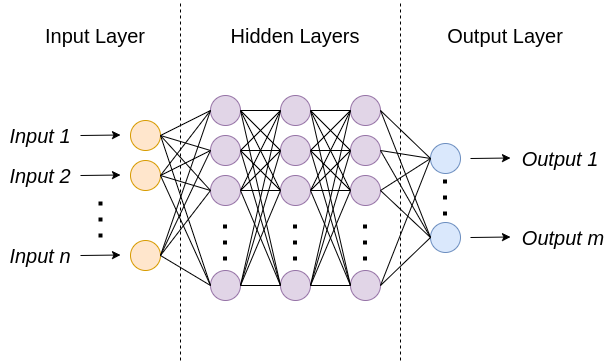
\includegraphics[width=.7\textwidth]{neural_network_sketch}
\caption[Sketch of a Neural Network]{
  \textbf{Sketch of a neural network.}
  The image shows a sketch of a neural network with three fully connected hidden layers. The network expects $n$ inputs and has $m$ possible outputs.
}
\label{fig:neural_network_sketch}
\end{figure}
Each neuron holds an associated weight and threshold. It receives an input and outputs the sum of weighted inputs. If this sum is greater than the associated threshold, the neuron gets activated.

A large part of the success of neural networks can be traced to the use of \textit{backpropagation}. Backpropagation uses information from the previous epoch (i.e. iteration) to adjust the weights of the network using the error gradient.

A neural network with one or more hidden layers defines a non-linear function. It is theoretically able to represent any function. Thus, neural networks are \textit{generic function approximators}. In addition, neural networks are highly expressive and flexible. They are applied successfully in many areas. However, neural networks also come with a few limitations or disadvantages. The backpropagation algorithm requires the calculation of an accurate gradient. Depending on the problem, this can be a challenging task. For example, calculating an accurate gradient in RL problems is usually non-trivial. Furthermore, there is a lack of understanding. The output of a neural network is often incomprehensible because of its complex structure.

\todo[inline]{Explain more, e.g. bias, feed forward neural network}



\subsection{Polynomial}
In mathematics, a polynomial is the sum of powers in one or more variables multiplied by constant coefficients. Given a field $F$, a polynomial in variable $x$ with coefficients in $F$ is a formal expression denoted by
\begin{align*}
  &f(x) = \Sigma_{i=0}^{n} a_i x^i \in F[x], &a_0, ..., a_n \in F, \ \ i \in \mathbb{N},
\end{align*}
where $F[x]$ represents the set of all such polynomials (\citet{fischer2014}, p. 61). The above formula shows the one dimensional case. For the multi-dimensional case, $x$ and the coefficients are vectors instead of scalars. Thus, a polynomial $p(\mathbf{x})$ with $\mathbf{x} = [x_0, ..., x_m]^T$ being a vector and of degree $n$ can be represented by
\begin{align*}
  &p(\mathbf{x}) = \Sigma_{i=0}^{n} \mathbf{w_i}^T (x_k^i)_{k \in I} \in F^n[\mathbf{x}], &\mathbf{w_0}, ... \mathbf{w_n} \in F^n, \ \ I = \{0, ..., m\}.
\end{align*}
Polynomials are relatively simple mathematical expressions and offer some significant advantages: their derivative and indefinite integral are easy to determine and are also polynomial. Due to their simple structure, polynomials can be valuable to analyze more complex functions using polynomial approximations. \textit{Taylor's theorem} tells us that we can locally approximate any $k$-times differentiable function by a polynomial of degree $k$. We call this approximation \textit{Taylor polynomial}. Furthermore, the \textit{Weierstrass approximation theorem} says that we can uniformly approximate every continuous function defined on a closed interval by a polynomial. Other applications of polynomials are \textit{polynomial interpolation} and \textit{polynomial splines}. Polynomial interpolation describes the problem of constructing a polynomial that passes through all given data points. Polynomial splines are piecewise polynomial functions that can be used for spline interpolation.

\todo[inline]{Include theorems (Taylor, Weierstass) \\ Explain difference between approximation and interpolation \\ Does $F^n$ make sense?}

\subsection{Fourier}

\subsection{Splines}
General splines, adjustments, Bézier curves maybe? 


\section{Previous Work}

\subsection{Benchmarks in Reinforcement Learning}
\label{ssec:benchmarks}
When developing a novel algorithm, it is important to compare our results with existing models. For this evaluation, we need standard benchmark problems. These are a set of standard optimization problems. OpenAI Gym \footnote{\url{gym.openai.com}} is a toolkit created for exactly this scenario. It contains a collection of benchmark problems with various levels of difficulty. However, not all benchmark problems are meaningful for the evaluation of an algorithm. If a problem is too trivial to solve, the results do not reflect the quality of the model adequately. We do not need to put a large amount of effort into the creation of a complex model for an easy-to-solve task.

In the paper \emph{Analyzing Reinforcement Learning Benchmarks with Random Weight Guessing} (\citet{oller_analyzing_2020}), the authors analyze and visualize the complexity of standard RL benchmarks based on score distribution. They tested their approach on the five Classic Control benchmark problems from the OpenAI Gym interface: \verb|CartPole|, \verb|Acrobot|, \verb|Pendulum|, \verb|MountainCar|, and \verb|MountainCarCon-| \verb|tinuous|. Given an RL environment, the authors conducted a fixed series of experiments. For these experiments, they used three neural network architectures ($N_{architectures}=3$): a network without any hidden layers (0 HL, 0 HU), a network with a single hidden layer of 4 units (1 HL, 4 HU), and a network with two hidden layers of 4 units each (2 HL, 4 HU). With these, they cover a variety of network models that are suited to solve the given tasks. The evaluation of the benchmark problems should be as objective as possible and should not include bias in the data. To achieve this, the authors did not include any learning opportunities for the network models. Instead, they chose the network weights i.i.d. from the standard normal distribution $\mathcal{N}(0,1)$ with Random Weight Guessing (RWG). This approach assures randomness and no directed learning. The goal of the paper was not to further analyze the network models but to investigate the benchmark problems themselves. With this in mind, they initialized $10^4$ samples ($N_{samples}=10^4$) with different random weights. The number of samples would be too large for a reasonable learning strategy. However, the large number of samples serves a different purpose than optimizing the results. Instead, the aim is to draw statistical conclusions. Each of these samples of a neural network represents a controller that maps observations to actions in the environment. Later in this thesis, I will explore function approximators other than neural networks representing the controller. In the paper, the authors tested the controllers for each environment during 20 independent episodes ($N_{episodes}=20$). For each episode, they saved the score in the score tensor $S$. Algorithm~\ref{alg:environment-evaluation} illustrates the procedure with pseudocode.

\begin{algorithm}
\caption{Evaluation process taken from \citet{oller_analyzing_2020}}
\begin{algorithmic}[1]
\State Initialize environment
\State Create array $S$ of size $N_{architectures} \times N_{samples} \times N_{episodes}$
\For{$n = 1,2,...,N_{samples}$}
    \State Sample NN weights randomly from $\mathcal{N}(0,1)$
    \For{$e=1,2,...,N_{episodes}$}
      \State Reset the environment
      \State Run episode with NN
      \State Store accured episode reward in $S_{a,n,e}$
    \EndFor
\EndFor
\end{algorithmic}
\label{alg:environment-evaluation}
\end{algorithm}

After the authors obtained the scores, they calculated the mean performance over all episodes from a sample and its variance. These statistics are significant insights. They can reveal how stable the network models are in completing a given task. A low mean value suggests that, in general, the network cannot complete the task. The variance gives us further insight into the score distribution. It illustrates how spread out the scores are from their respective mean score. A high value means that we have high variability. A controller is valuable if it can solve a specific task reliably and stable. Therefore, we strive for a high value for the mean and a low value for the variance. However, training a network with random weight guessing should generally not result in a stable controller. If this is the case, we can assume that the task to solve was too trivial and is not valuable for evaluation measurements. In the illustrations of the paper, the authors ranked the samples according to their mean scores. They then visualized their results with three plots: a log-scale histogram of the mean scores, a scatter plot of the sample scores over their rank, a scatter plot of score variance over the mean score.

I reproduced the results of the authors following the mentioned methodology. My findings for the environment \verb|CartPole| are displayed in Figure~\ref{fig:plots_reproduced}.
\begin{figure}[ht]
\centering
\begin{subfigure}{\textwidth}
  \centering
  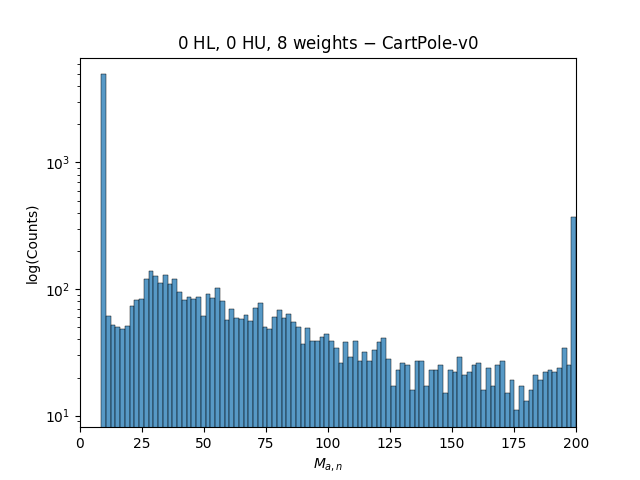
\includegraphics[width=0.329\textwidth]{reproduced_plots/HL_0_HU_0_histogram}
  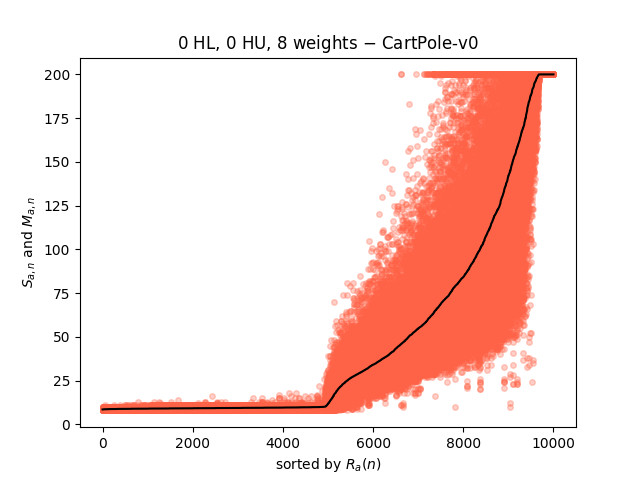
\includegraphics[width=0.329\textwidth]{reproduced_plots/HL_0_HU_0_scatter_score}
  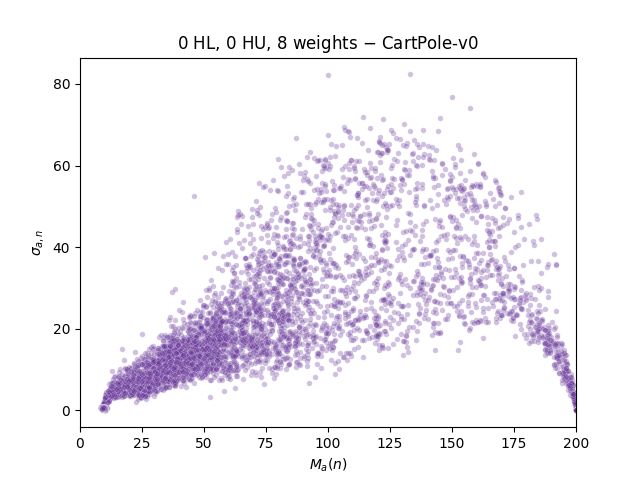
\includegraphics[width=0.329\textwidth]{reproduced_plots/HL_0_HU_0_scatter_variance}
    \caption{Results of network architecture without hidden layers}
    \label{fig:plots_reproduced_first}
\end{subfigure}
\begin{subfigure}{\textwidth}
  \centering
  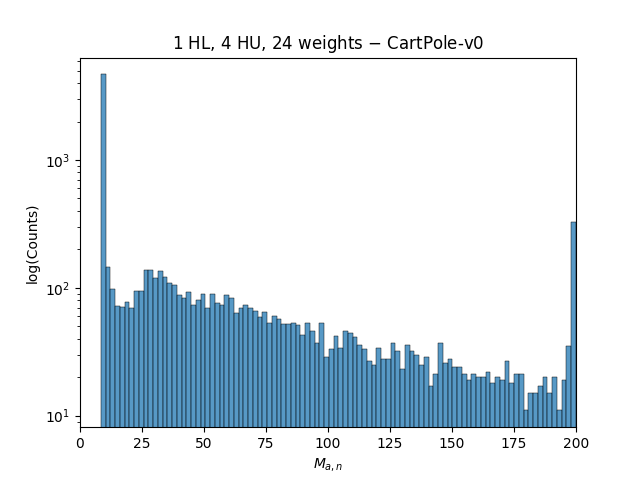
\includegraphics[width=0.329\textwidth]{reproduced_plots/HL_1_HU_4_histogram}
  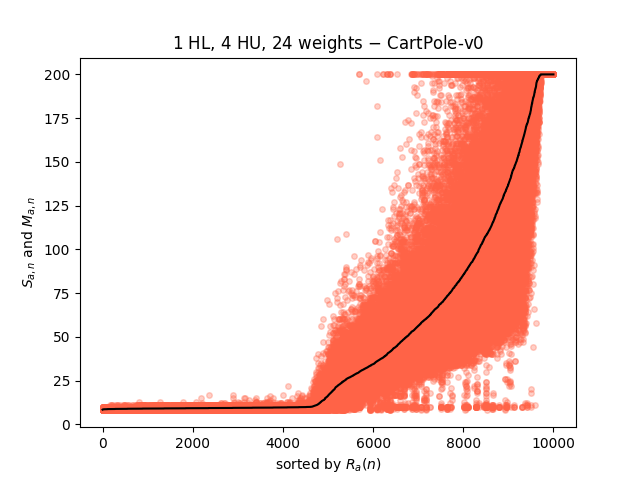
\includegraphics[width=0.329\textwidth]{reproduced_plots/HL_1_HU_4_scatter_score}
  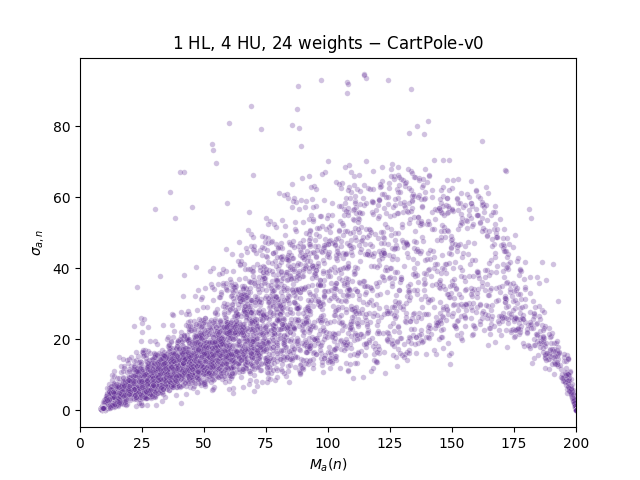
\includegraphics[width=0.329\textwidth]{reproduced_plots/HL_1_HU_4_scatter_variance}
    \caption{Results of network architecture with one hidden layer}
    \label{fig:plots_reproduced_second}
\end{subfigure}
\begin{subfigure}{\textwidth}
  \centering
  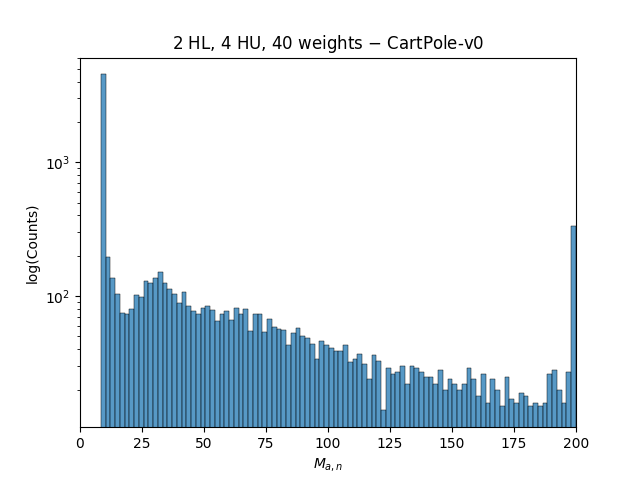
\includegraphics[width=0.329\textwidth]{reproduced_plots/HL_2_HU_4_histogram}
  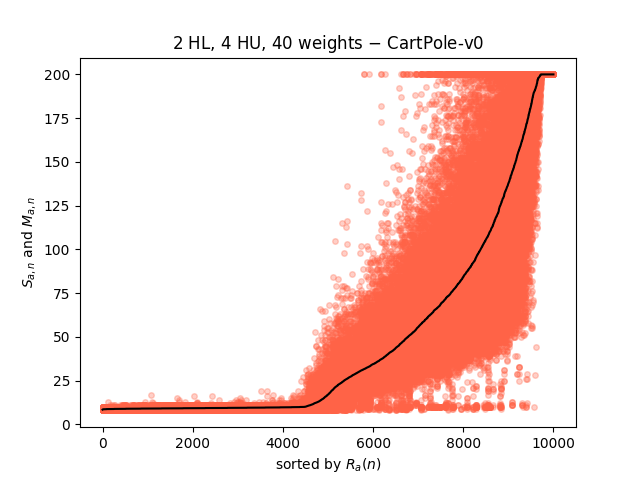
\includegraphics[width=0.329\textwidth]{reproduced_plots/HL_2_HU_4_scatter_score}
  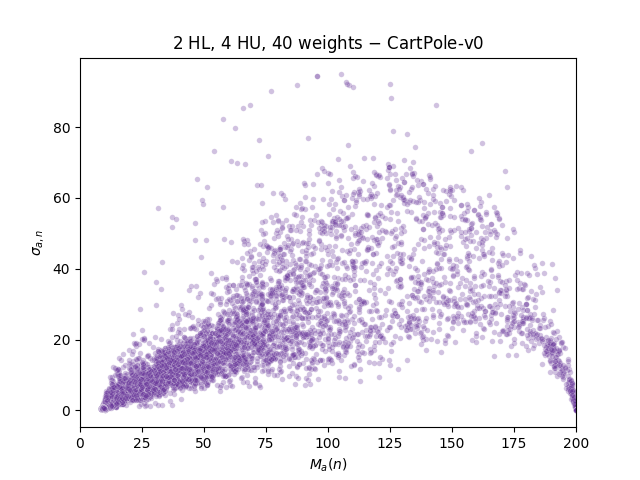
\includegraphics[width=0.329\textwidth]{reproduced_plots/HL_2_HU_4_scatter_variance}
    \caption{Results of network architecture with two hidden layers}
    \label{fig:plots_reproduced_third}
\end{subfigure}
\caption[Reproduced Plots]{
  \textbf{Results of the benchmark evaluation.}
   The plots show a log-scale histogram of the mean scores (left images), a scatter plot of the sample scores over their rank (middle images), a scatter plot of score variance over the mean score (right image). As expected with RWG, most networks were not able to solve the given task. However, there is still a significant amount of samples achieving a mean score of 200. That suggests that the environment is trivial to solve.
}
\label{fig:plots_reproduced}
\end{figure}
The plots illustrate the results for each of the three network architectures. Each row shows the histogram of the mean score values in the left image, the scatter plot of all scores over their rank in the image in the middle, and the scatter plot of the score variance over the mean score in the right image for a specific network architecture. There are few differences, but overall all network architectures deliver similar insights. The histogram plots show that the majority of networks receive a low score. Since the weights of the networks were chosen with RWG, this is rather unsurprising. But there is still a significant amount of networks that were able to achieve a high mean value or even the maximum value of 200. With a score of 200, the network was able to solve the task each episode. Therefore, the network could reliably solve the task without any learning technique involved. This should not be the case for a complex task. Furthermore, in the scatter plot in the middle, we can see that the line plot of the mean scores is a continuous increasing line without any jumps. Thus, a suited RL algorithm should generally be able to learn the task incrementally without converging into a local optimum. At the top of the scatter plot, we can see quite a few data points with a score of 200 that have a relatively low mean score. This indicates that a network that generally performs poorly can still solve the task with the right initialization conditions. Lastly, in the scatter plot on the right, we can see the distribution of the variance according to the mean value. On the left side, we have low scores of variance corresponding with a low mean value. These networks were consistently unable to achieve a high score. Without any training involved, we can expect most networks to be in this area. However, in the middle of the plot, the data points are spread out. For a high variance, the scores of a network differ highly from the mean value. Thus, we might get lucky and receive a high score depending on initialization conditions, but we might as well get a low score. These networks are inconsistent and unstable. On the right side of the scatter plot, we can see that the data points with a high mean value are mostly of low variance. Thus, to achieve a high mean value, the network needs consistency.

Interestingly, the usage of the bias had a relatively large impact on the performance of the network in my experiments. Without bias, the networks seem to achieve overall better scores. All plots in Figure~\ref{fig:plots_reproduced} illustrate the results without bias. For comparison, Figure~\ref{fig:comparison_bias} shows the results of a network with two hidden layers with the same configurations as before but this time including bias. As we can see, the networks with bias connections have a much lower score in general. The number of networks that can consistently solve the task also decreases significantly. In the paper, the authors noted that the probability mass of top-performers generally increases when dropping the bias connections for all tested environments. Thus, this is not an isolated observation. However, they did not investigate this behavior further as it was not the focus of their paper.
\begin{figure}[ht]
\centering
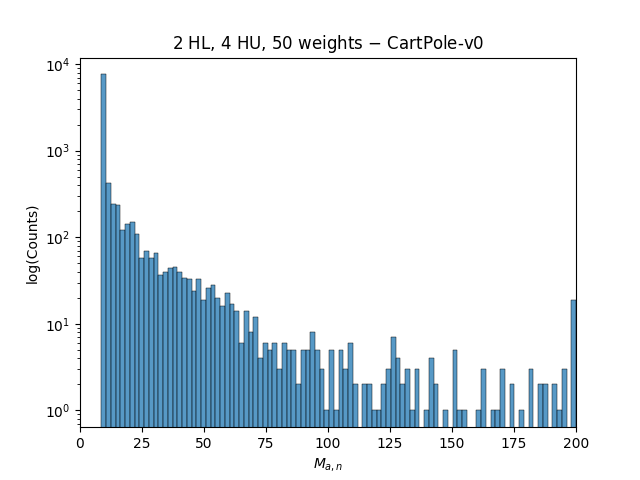
\includegraphics[width=0.329\textwidth]{with_bias_nn/HL_2_HU_4_histogram}
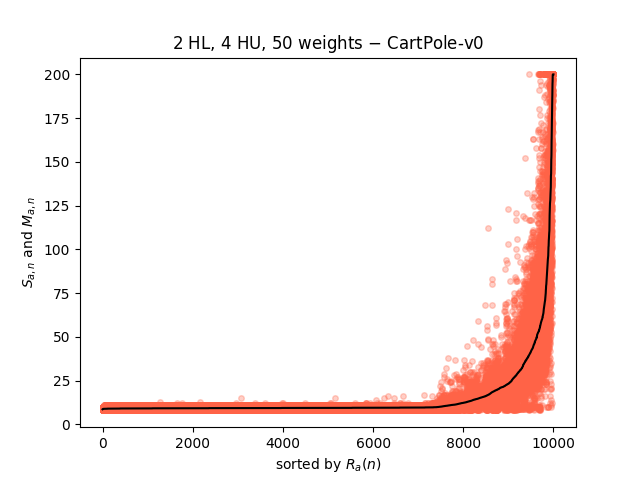
\includegraphics[width=0.329\textwidth]{with_bias_nn/HL_2_HU_4_scatter_score}
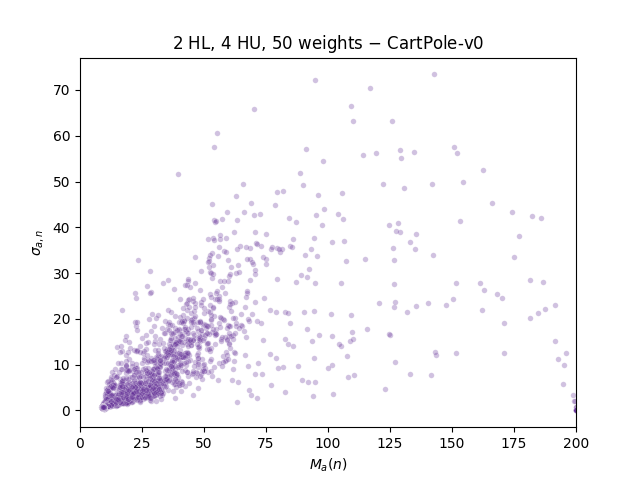
\includegraphics[width=0.329\textwidth]{with_bias_nn/HL_2_HU_4_scatter_variance}
\caption[Impact of Bias]{
  \textbf{Impact of bias.}
  The figures show the performance of a network with two hidden layers with the same settings as before but here we include bias. We can clearly see that the network with bias connection performs much worse than the one without.
}
\label{fig:comparison_bias}
\end{figure}
One possible explanation could be that guessing additional weights might be fatal for achieving a good score. Or in other words: the more possibilities we have to falsely guess a weight, the higher the probability to fail. To test this hypothesis, we can alter the number of weights and compare the results. With an increased number of weights, we would expect the networks to perform worse than before. However, it could also be that the number of weights is not as impactful as the complexity of the model in general. Randomly guessing the parameters of a simple model has a higher chance to result in a good (simple) model than guessing the parameters of a more complex model. The complexity of the network architecture gives an upper bound for the function that can be approximated. A network with high complexity maps into a larger search space with more complex functions. Since the size of the search space increases, there are also more possible samples that fail to solve the task. As the paper showed, a simple model is sufficient to solve these environments. A complex model is oversized for our purpose here. Thus, randomly guessing a simple model can yield a model with good performance with enough attempts. However, it is unlikely to randomly guess a complex model that performs well without any training involved. To test this hypothesis, we can increase the complexity of a network by varying the number of hidden layers or the number of neurons in a hidden layer. With increased complexity, we would expect the networks to perform worse than before.

Another interesting aspect would be to inspect the role of the bias in connection with the environments. A simple model is sufficient to solve a simple task. But what if the environment is more difficult to solve? In that case, the undersized complexity would limit us from finding an appropriate solution as the search space is not large enough for this scenario. Therefore, including bias should improve the results.

The experiments following this thought process are described in Chapter~\ref{ch:experiments}.


\todo[inline]{Add plots from Acrobot? \\ Make text easier to read with padding and more structure \\ Make captions of figures more meaningful (why is this added? why shown like this?), refer to subplots}

% \include{chapters/ ...}
% % !TEX root = ../main.tex

\chapter{Conclusion}
\label{ch:conclusions}

This work's driving question was whether we could find alternative models for reinforcement problems whose performance is comparable to the commonly used neural network model. To investigate how these models compare to neural networks and what advantages they have, two research questions were introduced in Section~\ref{sec:research_questions}. In addition, one research question was formulated concerning the architecture of a model for additional analysis.

\paragraph*{RQ1: How do function approximators other than neural networks compare with the latter?} In this work, I directly compared the alternative models, the polynomial and binary tree models, to neural networks. The polynomial model produced results comparable to those of neural networks. For the environment \verb|CartPole|, it delivered a more desirable score distribution for polynomials of degrees two and three. However, we would still prefer neural networks to tackle the problem of the \verb|Acrobot| environment. The environment \verb|MountainCar| seems to produce the same score distribution regardless of the model used. Thus, we cannot conclude that using the polynomial model robustly produces better results or results comparable to neural networks.

On the other hand, the binary tree model could deliver comparable results and even outperformed neural networks several times. The simplicity of the model did not limit the model's performance. The opposite is the case. It significantly outperformed neural networks for the environment \verb|CartPole|. Since \verb|CartPole| represents a relatively simple problem, the simple structure of binary trees is advantageous compared to the complex architecture of neural networks. Neural networks have proven that they are capable of solving many challenging problems. However, finding a good strategy with neural networks seems less efficient for a more straightforward task. The search space of the model can explain these results. A more complex model like neural networks with multiple hidden layers has a much larger search space in which they search for a good strategy for a given task. A large search space is a disadvantage when the task is easier to solve. Thus, we must carefully select our approach and adapt to the complexity of the task we want to solve.

The environment \verb|MountainCar| again produces a similar score distribution. The mean values seem to be identical. There are, however, a few higher individual scores for the binary tree model. As we can see in the results, the problem implemented in \verb|MountainCar| is hard to solve by RWG. All of the tested models showed similar findings. The large fitness plateau remains for all of them. To solve the problem, we need a learning algorithm high in exploration. For this use case, techniques in black-box optimization offer a good framework. Training a model with a learning algorithm prone to getting stuck in a local optimum will likely not result in a robust model that can solve the task. Also for the environment \verb|Acrobot|, the results of the two models look very similar. Although there are a few differences, both models seem equally suited to solve this task with the proper learning technique. Since a fitness plateau is present, an explorative learning algorithm should produce the best results.

Although the binary tree model only outputs discrete actions that are fixed, the results for the environment \verb|Pendulum| can compare to those of neural networks. Again, both models seem to be suited to solve the task reliably with an appropriate learning algorithm. In this case, the danger of being stuck in a local optimum is less prevalent than for the environment \verb|Acrobot|. Thus, the learning algorithm does not have to be as explorative. The environment \verb|MountainCarContiuous| delivered counterintuitive results. The restriction of the binary tree model to only output the two actions -1 and 1 from the otherwise continuous action space negatively influenced the model's performance. However, changing the actions from -1 and 1 to 0 and 1 resulted in a significantly better score distribution. Since the action defines the directional force applied to the car, a value between 0 and 1 means that we apply no force at all or actively push the car to the right in the direction of the target. Thus, the results show that the model does not necessarily have to learn to accelerate the car to the left and right to solve the task.

To conclude these findings, the binary tree model looks promising for problems in reinforcement learning. Combined with a suited learning technique, it should robustly produce results comparable to those of neural networks.

\paragraph*{RQ2: What advantages and disadvantages can we see with other function approximators?} With neural networks, we have many hyperparameters that need fine-tuning. We can completely change the model architecture by changing the number of layers or the number of neurons. We have to set many other components, like the activation function. In both the polynomial model and the binary tree model, we have only one parameter, namely the degree of the polynomial and the number of nodes of the binary tree. Thus, finding a suitable configuration of the architecture of the alternative is straightforward and does not need much effort as opposed to neural network models. In addition, the binary tree model offers much more insight into decision-making than the neural network model. To comprehend how a neural network makes a decision is very hard. The binary tree model offers much more interpretability in that sense.

\paragraph{RQ3: How does the bias influence the performance of the model?} Adding bias had a negative impact on all discrete models for the polynomial model and on almost all five classic control environments for the neural network model. In my experiments with the number of weights, the number of layers, and the number of neurons, none of these changes influenced the model's performance as much as the bias did. There seems to be something specific about the use of bias that changes the performance for these environments in the setting of RWG. Why this is the case needs further research. However, there are two exceptions. The environment \verb|MountainCarContiuous| was very reactive to each change in the architecture or the number of weights. The environment \verb|Pendulum| did not show a significant difference when using bias vs. when not using bias. A change in the architecture or the number of weights affected it similarly.


\section{Future Work}
There is much further research that can be done in this area. This work represents the first step in the direction of alternative models like the binary tree model. This thesis showed that the binary tree model looks promising and can produce results comparable to neural networks while maintaining a simple architecture and interpretability. However, it would be interesting how we can adapt the model to work better on specific problems. The current implementation of the model can undoubtedly be improved. For continuous action spaces, we can adapt the leaf nodes to be included in the learning algorithm or implement a function instead of outputting a fixed action.

So far, no practical learning technique has been involved. It would be interesting to see how the model performs with CMA-ES instead of RWG. Additionally, the model should be tested in more challenging benchmark problems like the environment \verb|BipedalWalker| also included in the set of environments provided by the OpenAI Gym interface.

Finally, it would be interesting to see how other models perform in this setting. With techniques in black-box optimization, there are numerous possibilities. For example, we could use an adapted version of the Fourier transform.

% didn't work with include, input works
% !TEX root = ../main.tex

\chapter{Introduction}
\label{ch:introduction}

\section{General Notation}
First, I am defining the notation I used throughout this thesis. For the scalars, I used regular, normal-weight variables such as $x$. Vectors are represented by bold lower-case variables like $\mathbf{x}$. Tensors and matrices are denoted by bold upper-case characters, such as $\mathbf{X}$. In summary:
\begin{align*}
x&: \text{Scalar} \\
\mathbf{x}&: \text{Vector} \\
\mathbf{X}&: \text{Matrix or tensor}
\end{align*}
\todo[inline]{Useful? Everything covered?}


\section{Black-Box Optimization}
\subsection{Evolution Strategies}
Evolution Strategies (ES) ...

\subsection{Covariance Matrix Adaptation Evolution Strategy}
Covariance Matrix Adaptation Evolution Strategy (CMA-ES) ...

\section{Function Approximators}
We can represent many problems in machine learning as a function mapping an input space into an output space. The output space or \textit{search space} denotes the space of all feasible solutions. The underlying function is the output of the learning process of an algorithm and is often called the \textit{target function}. Optimally, we would derive the formula of the function explicitly. However, even though we suspect that such a function exists, we usually do not have enough information to derive a formula directly. Thus, we aim to approximate the target function with \textit{function approximators} by using the available data. In general, we can apply any function approximator. However, each function approximator has its advantages and limitations. For example, some may be prone to local optimum. Depending on the task, this could prevent us from finding a good solution.

\subsection{Neural Networks}
Neural networks are machine learning algorithms inspired by the functionalities of the human brain. They consist of connected neurons or nodes that imitate the biological neurons of the brain sending signals to each other. A neuron receives one or multiple input values and calculates one or multiple output values. Figure [insert figure] illustrates one neuron. The neuron receives three input values and calculates one output value. For the caluclation of the ouptut, the neurons uses the assigned weights $w$. Thus, the output represents the sum of weighted inputs.

In a neural network, the neurons are arranged in connected layers. A network has at least an input and an output layer. We can further expand it with one or more hidden layers. Depending on the model, the connectivity between the layers differs. Figure~\ref{fig:neural_network_sketch} shows a sketch of a network with three hidden layers that are fully connected.
\begin{figure}[ht]
\centering
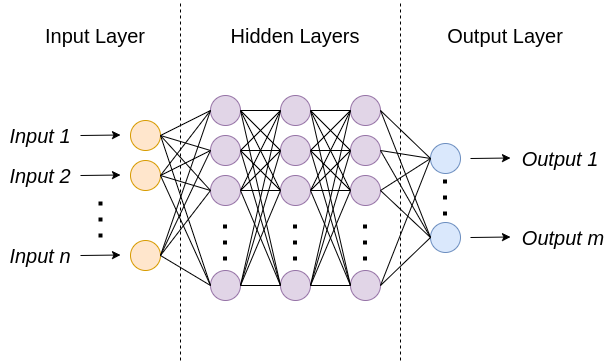
\includegraphics[width=.7\textwidth]{neural_network_sketch}
\caption[Sketch of a Neural Network]{
  \textbf{Sketch of a neural network.}
  The image shows a sketch of a neural network with three fully connected hidden layers. The network expects $n$ inputs and has $m$ possible outputs.
}
\label{fig:neural_network_sketch}
\end{figure}
Each neuron holds an associated weight and threshold. It receives an input and outputs the sum of weighted inputs. If this sum is greater than the associated threshold, the neuron gets activated.

A large part of the success of neural networks can be traced to the use of \textit{backpropagation}. Backpropagation uses information from the previous epoch (i.e. iteration) to adjust the weights of the network using the error gradient.

A neural network with one or more hidden layers defines a non-linear function. It is theoretically able to represent any function. Thus, neural networks are \textit{generic function approximators}. In addition, neural networks are highly expressive and flexible. They are applied successfully in many areas. However, neural networks also come with a few limitations or disadvantages. The backpropagation algorithm requires the calculation of an accurate gradient. Depending on the problem, this can be a challenging task. For example, calculating an accurate gradient in RL problems is usually non-trivial. Furthermore, there is a lack of understanding. The output of a neural network is often incomprehensible because of its complex structure.

\todo[inline]{Explain more, e.g. bias, feed forward neural network}



\subsection{Polynomial}
In mathematics, a polynomial is the sum of powers in one or more variables multiplied by constant coefficients. Given a field $F$, a polynomial in variable $x$ with coefficients in $F$ is a formal expression denoted by
\begin{align*}
  &f(x) = \Sigma_{i=0}^{n} a_i x^i \in F[x], &a_0, ..., a_n \in F, \ \ i \in \mathbb{N},
\end{align*}
where $F[x]$ represents the set of all such polynomials (\citet{fischer2014}, p. 61). The above formula shows the one dimensional case. For the multi-dimensional case, $x$ and the coefficients are vectors instead of scalars. Thus, a polynomial $p(\mathbf{x})$ with $\mathbf{x} = [x_0, ..., x_m]^T$ being a vector and of degree $n$ can be represented by
\begin{align*}
  &p(\mathbf{x}) = \Sigma_{i=0}^{n} \mathbf{w_i}^T (x_k^i)_{k \in I} \in F^n[\mathbf{x}], &\mathbf{w_0}, ... \mathbf{w_n} \in F^n, \ \ I = \{0, ..., m\}.
\end{align*}
Polynomials are relatively simple mathematical expressions and offer some significant advantages: their derivative and indefinite integral are easy to determine and are also polynomial. Due to their simple structure, polynomials can be valuable to analyze more complex functions using polynomial approximations. \textit{Taylor's theorem} tells us that we can locally approximate any $k$-times differentiable function by a polynomial of degree $k$. We call this approximation \textit{Taylor polynomial}. Furthermore, the \textit{Weierstrass approximation theorem} says that we can uniformly approximate every continuous function defined on a closed interval by a polynomial. Other applications of polynomials are \textit{polynomial interpolation} and \textit{polynomial splines}. Polynomial interpolation describes the problem of constructing a polynomial that passes through all given data points. Polynomial splines are piecewise polynomial functions that can be used for spline interpolation.

\todo[inline]{Include theorems (Taylor, Weierstass) \\ Explain difference between approximation and interpolation \\ Does $F^n$ make sense?}

\subsection{Fourier}

\subsection{Splines}
General splines, adjustments, Bézier curves maybe? 


\section{Previous Work}

\subsection{Benchmarks in Reinforcement Learning}
\label{ssec:benchmarks}
When developing a novel algorithm, it is important to compare our results with existing models. For this evaluation, we need standard benchmark problems. These are a set of standard optimization problems. OpenAI Gym \footnote{\url{gym.openai.com}} is a toolkit created for exactly this scenario. It contains a collection of benchmark problems with various levels of difficulty. However, not all benchmark problems are meaningful for the evaluation of an algorithm. If a problem is too trivial to solve, the results do not reflect the quality of the model adequately. We do not need to put a large amount of effort into the creation of a complex model for an easy-to-solve task.

In the paper \emph{Analyzing Reinforcement Learning Benchmarks with Random Weight Guessing} (\citet{oller_analyzing_2020}), the authors analyze and visualize the complexity of standard RL benchmarks based on score distribution. They tested their approach on the five Classic Control benchmark problems from the OpenAI Gym interface: \verb|CartPole|, \verb|Acrobot|, \verb|Pendulum|, \verb|MountainCar|, and \verb|MountainCarCon-| \verb|tinuous|. Given an RL environment, the authors conducted a fixed series of experiments. For these experiments, they used three neural network architectures ($N_{architectures}=3$): a network without any hidden layers (0 HL, 0 HU), a network with a single hidden layer of 4 units (1 HL, 4 HU), and a network with two hidden layers of 4 units each (2 HL, 4 HU). With these, they cover a variety of network models that are suited to solve the given tasks. The evaluation of the benchmark problems should be as objective as possible and should not include bias in the data. To achieve this, the authors did not include any learning opportunities for the network models. Instead, they chose the network weights i.i.d. from the standard normal distribution $\mathcal{N}(0,1)$ with Random Weight Guessing (RWG). This approach assures randomness and no directed learning. The goal of the paper was not to further analyze the network models but to investigate the benchmark problems themselves. With this in mind, they initialized $10^4$ samples ($N_{samples}=10^4$) with different random weights. The number of samples would be too large for a reasonable learning strategy. However, the large number of samples serves a different purpose than optimizing the results. Instead, the aim is to draw statistical conclusions. Each of these samples of a neural network represents a controller that maps observations to actions in the environment. Later in this thesis, I will explore function approximators other than neural networks representing the controller. In the paper, the authors tested the controllers for each environment during 20 independent episodes ($N_{episodes}=20$). For each episode, they saved the score in the score tensor $S$. Algorithm~\ref{alg:environment-evaluation} illustrates the procedure with pseudocode.

\begin{algorithm}
\caption{Evaluation process taken from \citet{oller_analyzing_2020}}
\begin{algorithmic}[1]
\State Initialize environment
\State Create array $S$ of size $N_{architectures} \times N_{samples} \times N_{episodes}$
\For{$n = 1,2,...,N_{samples}$}
    \State Sample NN weights randomly from $\mathcal{N}(0,1)$
    \For{$e=1,2,...,N_{episodes}$}
      \State Reset the environment
      \State Run episode with NN
      \State Store accured episode reward in $S_{a,n,e}$
    \EndFor
\EndFor
\end{algorithmic}
\label{alg:environment-evaluation}
\end{algorithm}

After the authors obtained the scores, they calculated the mean performance over all episodes from a sample and its variance. These statistics are significant insights. They can reveal how stable the network models are in completing a given task. A low mean value suggests that, in general, the network cannot complete the task. The variance gives us further insight into the score distribution. It illustrates how spread out the scores are from their respective mean score. A high value means that we have high variability. A controller is valuable if it can solve a specific task reliably and stable. Therefore, we strive for a high value for the mean and a low value for the variance. However, training a network with random weight guessing should generally not result in a stable controller. If this is the case, we can assume that the task to solve was too trivial and is not valuable for evaluation measurements. In the illustrations of the paper, the authors ranked the samples according to their mean scores. They then visualized their results with three plots: a log-scale histogram of the mean scores, a scatter plot of the sample scores over their rank, a scatter plot of score variance over the mean score.

I reproduced the results of the authors following the mentioned methodology. My findings for the environment \verb|CartPole| are displayed in Figure~\ref{fig:plots_reproduced}.
\begin{figure}[ht]
\centering
\begin{subfigure}{\textwidth}
  \centering
  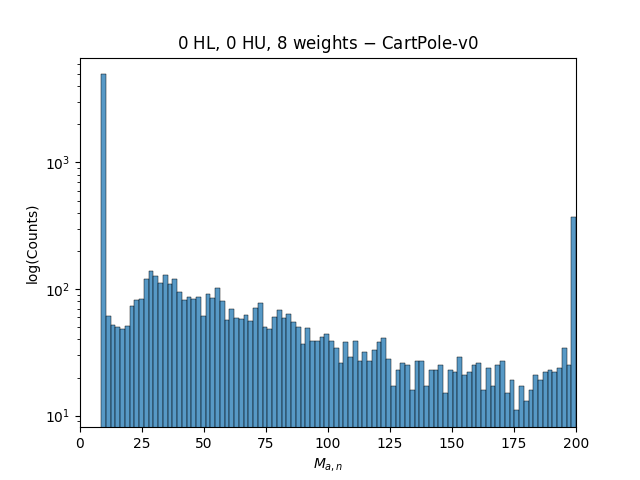
\includegraphics[width=0.329\textwidth]{reproduced_plots/HL_0_HU_0_histogram}
  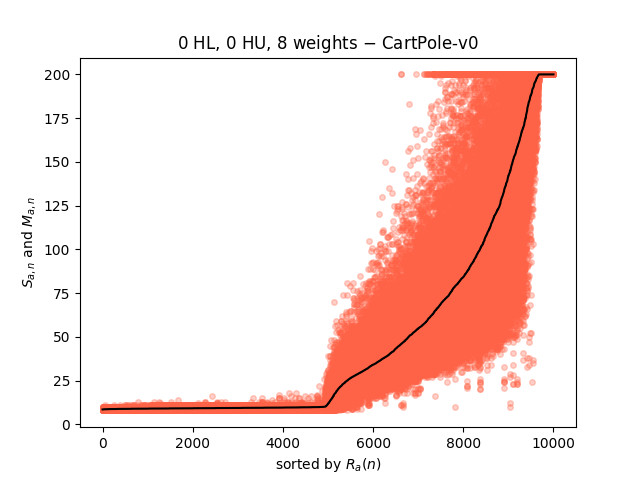
\includegraphics[width=0.329\textwidth]{reproduced_plots/HL_0_HU_0_scatter_score}
  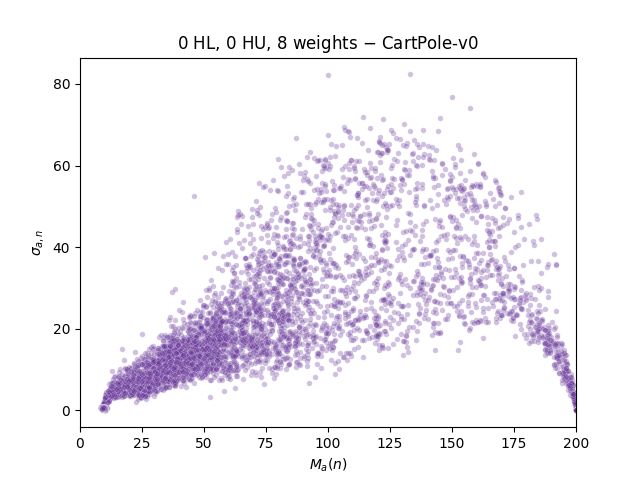
\includegraphics[width=0.329\textwidth]{reproduced_plots/HL_0_HU_0_scatter_variance}
    \caption{Results of network architecture without hidden layers}
    \label{fig:plots_reproduced_first}
\end{subfigure}
\begin{subfigure}{\textwidth}
  \centering
  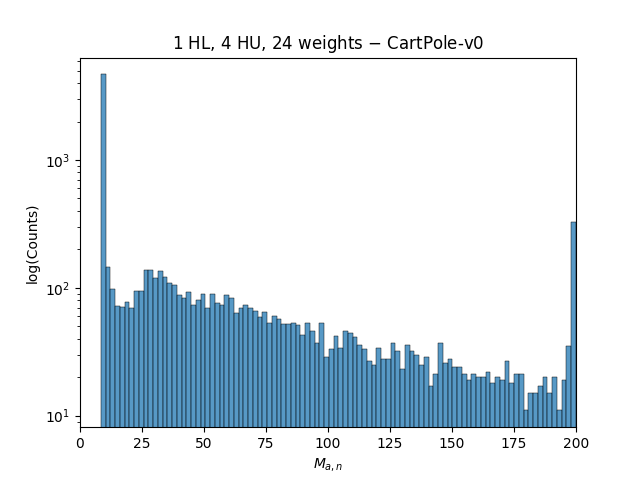
\includegraphics[width=0.329\textwidth]{reproduced_plots/HL_1_HU_4_histogram}
  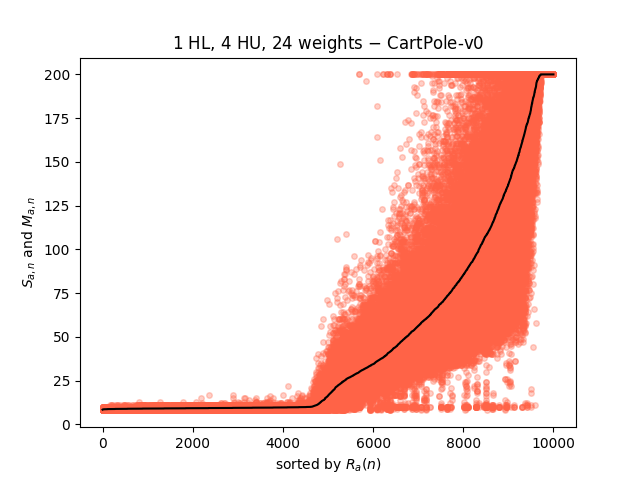
\includegraphics[width=0.329\textwidth]{reproduced_plots/HL_1_HU_4_scatter_score}
  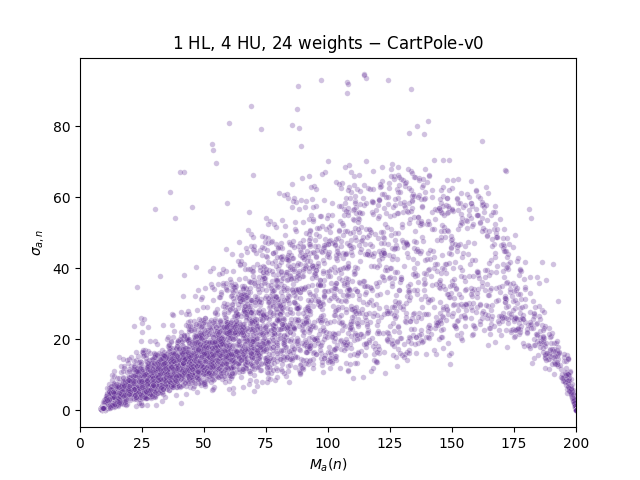
\includegraphics[width=0.329\textwidth]{reproduced_plots/HL_1_HU_4_scatter_variance}
    \caption{Results of network architecture with one hidden layer}
    \label{fig:plots_reproduced_second}
\end{subfigure}
\begin{subfigure}{\textwidth}
  \centering
  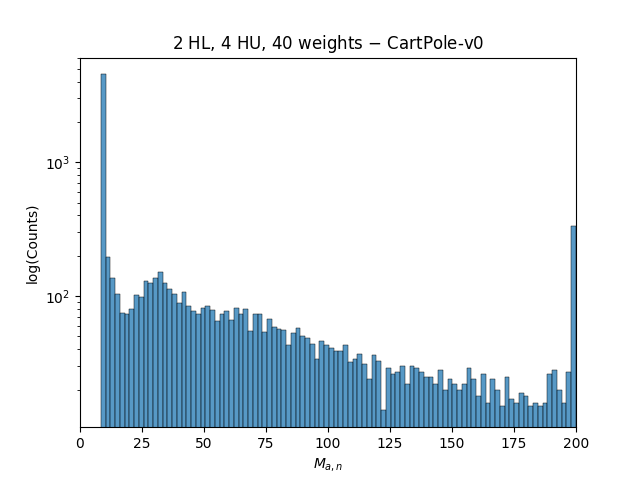
\includegraphics[width=0.329\textwidth]{reproduced_plots/HL_2_HU_4_histogram}
  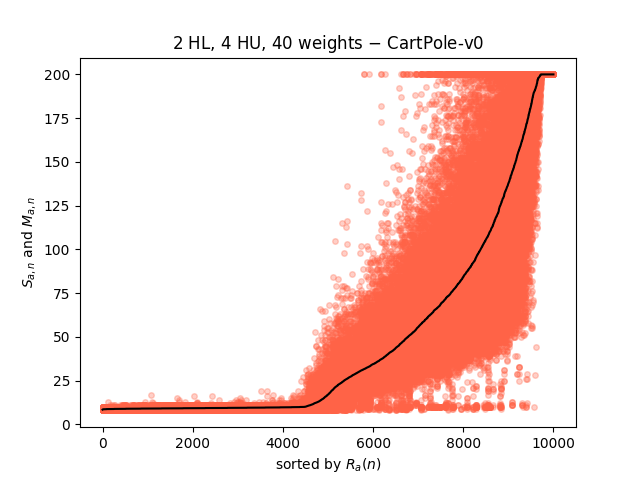
\includegraphics[width=0.329\textwidth]{reproduced_plots/HL_2_HU_4_scatter_score}
  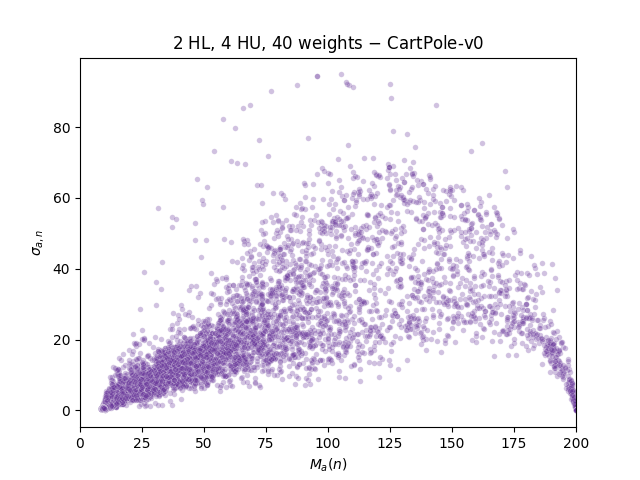
\includegraphics[width=0.329\textwidth]{reproduced_plots/HL_2_HU_4_scatter_variance}
    \caption{Results of network architecture with two hidden layers}
    \label{fig:plots_reproduced_third}
\end{subfigure}
\caption[Reproduced Plots]{
  \textbf{Results of the benchmark evaluation.}
   The plots show a log-scale histogram of the mean scores (left images), a scatter plot of the sample scores over their rank (middle images), a scatter plot of score variance over the mean score (right image). As expected with RWG, most networks were not able to solve the given task. However, there is still a significant amount of samples achieving a mean score of 200. That suggests that the environment is trivial to solve.
}
\label{fig:plots_reproduced}
\end{figure}
The plots illustrate the results for each of the three network architectures. Each row shows the histogram of the mean score values in the left image, the scatter plot of all scores over their rank in the image in the middle, and the scatter plot of the score variance over the mean score in the right image for a specific network architecture. There are few differences, but overall all network architectures deliver similar insights. The histogram plots show that the majority of networks receive a low score. Since the weights of the networks were chosen with RWG, this is rather unsurprising. But there is still a significant amount of networks that were able to achieve a high mean value or even the maximum value of 200. With a score of 200, the network was able to solve the task each episode. Therefore, the network could reliably solve the task without any learning technique involved. This should not be the case for a complex task. Furthermore, in the scatter plot in the middle, we can see that the line plot of the mean scores is a continuous increasing line without any jumps. Thus, a suited RL algorithm should generally be able to learn the task incrementally without converging into a local optimum. At the top of the scatter plot, we can see quite a few data points with a score of 200 that have a relatively low mean score. This indicates that a network that generally performs poorly can still solve the task with the right initialization conditions. Lastly, in the scatter plot on the right, we can see the distribution of the variance according to the mean value. On the left side, we have low scores of variance corresponding with a low mean value. These networks were consistently unable to achieve a high score. Without any training involved, we can expect most networks to be in this area. However, in the middle of the plot, the data points are spread out. For a high variance, the scores of a network differ highly from the mean value. Thus, we might get lucky and receive a high score depending on initialization conditions, but we might as well get a low score. These networks are inconsistent and unstable. On the right side of the scatter plot, we can see that the data points with a high mean value are mostly of low variance. Thus, to achieve a high mean value, the network needs consistency.

Interestingly, the usage of the bias had a relatively large impact on the performance of the network in my experiments. Without bias, the networks seem to achieve overall better scores. All plots in Figure~\ref{fig:plots_reproduced} illustrate the results without bias. For comparison, Figure~\ref{fig:comparison_bias} shows the results of a network with two hidden layers with the same configurations as before but this time including bias. As we can see, the networks with bias connections have a much lower score in general. The number of networks that can consistently solve the task also decreases significantly. In the paper, the authors noted that the probability mass of top-performers generally increases when dropping the bias connections for all tested environments. Thus, this is not an isolated observation. However, they did not investigate this behavior further as it was not the focus of their paper.
\begin{figure}[ht]
\centering
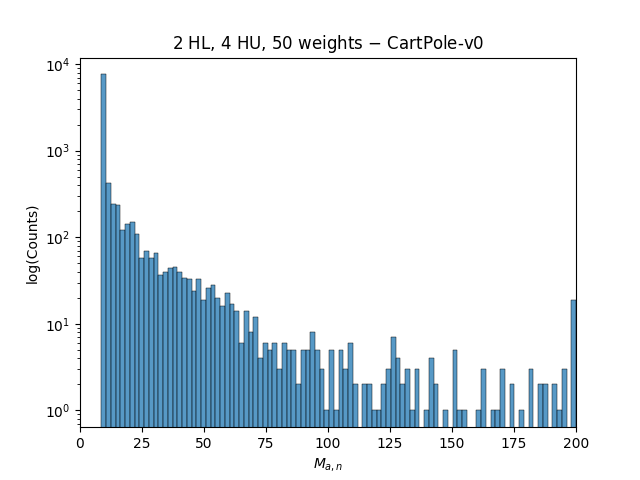
\includegraphics[width=0.329\textwidth]{with_bias_nn/HL_2_HU_4_histogram}
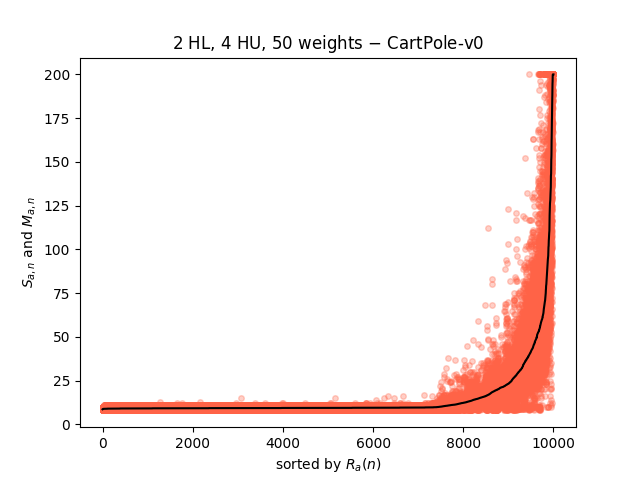
\includegraphics[width=0.329\textwidth]{with_bias_nn/HL_2_HU_4_scatter_score}
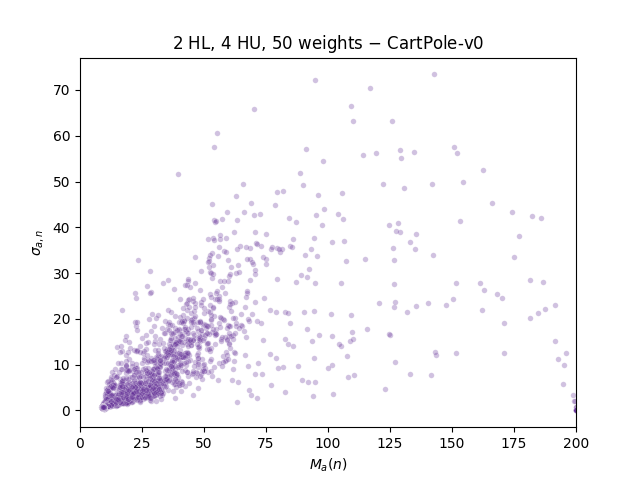
\includegraphics[width=0.329\textwidth]{with_bias_nn/HL_2_HU_4_scatter_variance}
\caption[Impact of Bias]{
  \textbf{Impact of bias.}
  The figures show the performance of a network with two hidden layers with the same settings as before but here we include bias. We can clearly see that the network with bias connection performs much worse than the one without.
}
\label{fig:comparison_bias}
\end{figure}
One possible explanation could be that guessing additional weights might be fatal for achieving a good score. Or in other words: the more possibilities we have to falsely guess a weight, the higher the probability to fail. To test this hypothesis, we can alter the number of weights and compare the results. With an increased number of weights, we would expect the networks to perform worse than before. However, it could also be that the number of weights is not as impactful as the complexity of the model in general. Randomly guessing the parameters of a simple model has a higher chance to result in a good (simple) model than guessing the parameters of a more complex model. The complexity of the network architecture gives an upper bound for the function that can be approximated. A network with high complexity maps into a larger search space with more complex functions. Since the size of the search space increases, there are also more possible samples that fail to solve the task. As the paper showed, a simple model is sufficient to solve these environments. A complex model is oversized for our purpose here. Thus, randomly guessing a simple model can yield a model with good performance with enough attempts. However, it is unlikely to randomly guess a complex model that performs well without any training involved. To test this hypothesis, we can increase the complexity of a network by varying the number of hidden layers or the number of neurons in a hidden layer. With increased complexity, we would expect the networks to perform worse than before.

Another interesting aspect would be to inspect the role of the bias in connection with the environments. A simple model is sufficient to solve a simple task. But what if the environment is more difficult to solve? In that case, the undersized complexity would limit us from finding an appropriate solution as the search space is not large enough for this scenario. Therefore, including bias should improve the results.

The experiments following this thought process are described in Chapter~\ref{ch:experiments}.


\todo[inline]{Add plots from Acrobot? \\ Make text easier to read with padding and more structure \\ Make captions of figures more meaningful (why is this added? why shown like this?), refer to subplots}

% !TEX root = ../main.tex

\chapter{Experiments}
\label{ch:experiments}

\section{Research Questions}
To analyze and compare the different models and their architectures, I formulated the following research questions:
\begin{enumerate}
  \item How do function approximators other than neural networks compare with the latter?
  \item Why did the models without bias generally perform better than the ones with bias?
  \begin{enumerate}
    \item Does increasing the number of weights worsen the performance of the model?
    \item Does a neural network with more than two hidden layers yield worse scores?
    \item Does the neural network's performance suffer from an increase in the number of neurons?
  \end{enumerate}
\end{enumerate}

\section{Experiments}
To investigate and answer the formulated research questions, I conducted the following experiments:
\begin{enumerate}
  \item I selected a few promising models to analyze. They are described in Section~\ref{ssec:models}. Similar to \citet{oller_analyzing_2020}, I used RWG to draw the weights of the models and tested the performance on a Classic Control environment from OpenAI Gym.
  \item With the same settings for the experiments as in Section~\ref{ssec:benchmarks}, I varied the number of (a) weights, (b) hidden layers, and (c) neurons for a neural network and compared the results.
\end{enumerate}

\subsection{Experiment 1}
In the first experiment, analogous to \citet{oller_analyzing_2020}, there is no learning involved. For their paper, they were interested in the complexity of the environment, whereas I aim to find out more about the nature of the models. I selected a few candidates for the models, which are described in Section~\ref{ssec:models} and used them for a series of experiments. I used the same procedure for all models, which allows me to compare them with one another. For the experiments, first, I initialized the environment. I used the \verb|CartPole| and \verb|Acrobot| environment for these experiments. These environments are fairly easy to solve, as explained in Section~\ref{ssec:benchmarks}. Therefore, we expect some controllers to solve the task even without any training. Second, I initialized the respective model. Then, I drew the model weights from the standard normal distribution $\mathcal{N}(0,1)$. Each of these instances of the model represents a sample. In total, I used $10'000$ samples ($N_{samples}$). Finally, I ran 20 episodes ($N_{episodes}$) with each sample for an environment and stored the respective score as an entry of the score tensor $S$. Algorithm~\ref{alg:model-evaluation} shows an overview of the described procedure.
\begin{algorithm}
\caption{First experiment with RWG}
\begin{algorithmic}[1]
\State Initialize environment
\State Initialize model
\State Create array $S$ of size $N_{samples} \times N_{episodes}$
\For{$n = 1,2,...,N_{samples}$}
    \State Sample model weights randomly from $\mathcal{N}(0,1)$
    \For{$e=1,2,...,N_{episodes}$}
      \State Reset the environment
      \State Run episode with model
      \State Store accured episode reward in $S_{n,e}$
    \EndFor
\EndFor
\end{algorithmic}
\label{alg:model-evaluation}
\end{algorithm}

\subsection{Experiment 2}
For the second experiment, I used the same procedure as described in Section~\ref{ssec:benchmarks}. I used neural networks for all experiments. Additionally, I used the polynomial model for the experiment concerning the weights of the model.
\begin{enumerate}
  \item I used the same number of hidden layers and neurons for the neural networks as before: a network without hidden layers, a network with one hidden layer with four hidden units, and a network with two hidden layers and four hidden units for each layer. I only changed the number of weights for each network. In addition, I used the model $P_1$ described in Section~\ref{ssec:models}.

  First, I doubled the number of weights for all models. Then, I tripled the number of weights for all models. To achieve this, I constructed one weight $\mathbf{w_i}$ out of two, respectively, three weights by addition:
  \begin{align*}
    &\text{Double number of weights: } &\mathbf{w_i} &= \mathbf{w_{i1}} + \mathbf{w_{i2}} \\
    &\text{Triple number of weights: } &\mathbf{w_{i}} &= \mathbf{w_{i1}} + \mathbf{w_{i2}} + \mathbf{w_{i3}}
  \end{align*}
  \item In this experiment, I tested the models with different numbers of hidden layers. Each layer still has the same number of hidden neurons as before. Thus, the networks have four hidden units for each layer. I used a network with four hidden layers, one with six, and one with eight.
  \item For this experiment, I varied the number of hidden neurons for a network. I used a network with two hidden layers. For the number of hidden neurons, I chose 5, 8, and 10.
\end{enumerate}
\todo[inline]{Maybe add table with used architecture to make it more comprehensible}

\subsection{OpenAI Gym Environments}
\begin{itemize}
  \item CartPole
  \item Acrobot
\end{itemize}

\todo[inline]{Explain used environments}

\subsection{Models}
\label{ssec:models}
For the polynomial model, I used two architectures $P_1$ and $P_2$. The first model $P_1$ consists of one polynomial for each possible action in a discrete action space. The input of the model is the observation from the environment. The dimension of the weight vectors is according to the dimension of the input vector. For the environment \verb|CartPole| with the discrete action space $\{0, 1\}$ and observation $\mathbf{x} = [x_0, x_1, x_2, x_3]^T$, this means that $P_1$ consists of two polynomials:
\begin{align*}
  &p_0(\mathbf{x}) = \Sigma_{i=0}^{n} \mathbf{w_i}^T (x_k^i)_{k \in I} \in \mathbb{R}, &\mathbf{w_0}, ..., \mathbf{w_3}, \mathbf{x} \in \mathbb{R}^4, \ \ I = \{0, 1, 2, 3\} \\
  &p_1(\mathbf{x}) = \Sigma_{i=0}^{n} \mathbf{\hat{w}_i}^T (x_k^i)_{k \in I} \in \mathbb{R}, &\mathbf{\hat{w}_0}, ..., \mathbf{\hat{w}_3}, \mathbf{x} \in \mathbb{R}^4, \ \ I = \{0, 1, 2, 3\}
\end{align*}
In the formulas, $n$ denotes the degree of the polynomial. In my experiments, I tested polynomials of degrees 1, 2, and 3. The output of the polynomials has no reasonable upper and lower limit, as illustrated in Figure~\ref{fig:bounds}. That makes it harder to interpret the results reasonably.
\begin{figure}[ht]
\centering
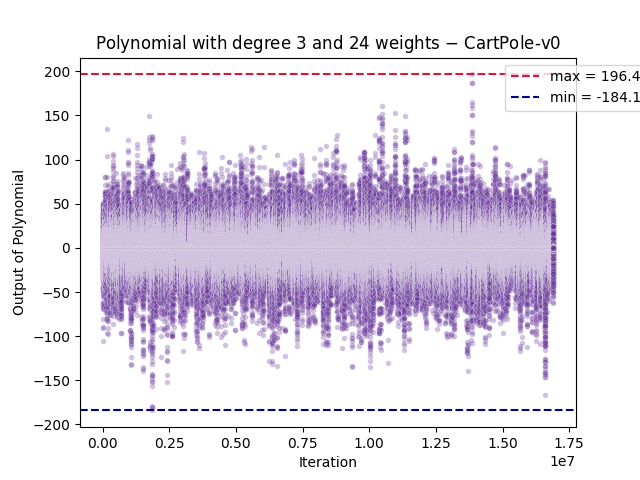
\includegraphics[width=0.6\textwidth]{PolynomialNN_degree_3_bounds}
\caption[Upper and lower bound]{
  \textbf{Upper and lower bound.}
  The figure shows each output of the polynomial functions described above. As we can see, the functions are not well bound, and there are quite a few outliers. That makes it hard to interpret the output sensibly.
}
\label{fig:bounds}
\end{figure}
So, I scaled the outputs with a sigmoid function. A sigmoid function is a mathematical function that maps an arbitrary input space into an output space with a small range, for example, 0 and 1. The function has a characteristic S-shaped curve. We can interpret the output space of the sigmoid function as a probability. In this case, we search for the probability that a specific action is the reasonable one given an observation $\mathbf{x}$. Thus, for our example with the \verb|CartPole| environment, we can interpret $sig(p_0)$ as the probability that action 0 is the correct one and $sig(p_1)$ as the probability that action 1 is the correct one. Putting this thought into a formula for $P_1$ and the \verb|CartPole| environment, we get:
\[
  P_1(\mathbf{x}) =
  \begin{cases}1~&{\text{ if }}~sig(p_1(\mathbf{x})) > sig(p_0(\mathbf{x}))~,\\0~&~\text{otherwise}~.\end{cases}
\]
For the sigmoid function, I used the logistic sigmoid function. The formula and a plot of the function in 2D are shown in Figure~\ref{fig:sigmoid}.
\begin{figure}[ht]
\centering
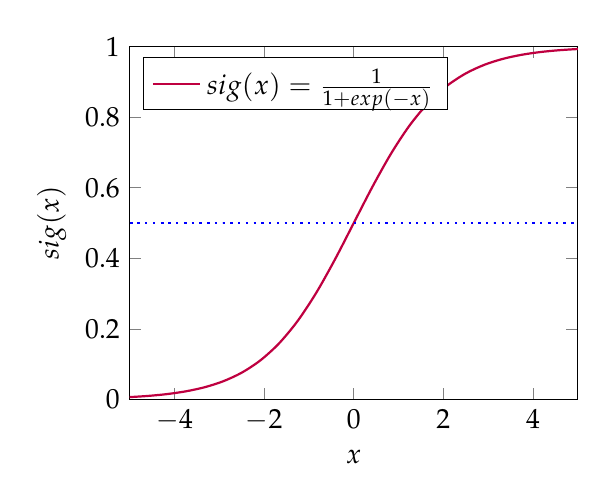
\begin{tikzpicture}
\begin{axis}[
      xmin = -5, xmax = 5,
      ymin = 0, ymax = 1,
      legend cell align = {left},
      legend pos = north west,
      width = 0.6\textwidth,
      height = 0.5\textwidth,
      xlabel = \(x\),
      ylabel = {\(sig(x)\)}
    ]
    \addplot[
        smooth,
        thick,
        purple
    ] {1 / (1 + exp(-x))};
    \addlegendentry{
    $sig(x) = \frac{1}{1 + exp(-x)}$
    }
    \addplot[
        smooth,
        thick,
        blue,
        dotted
    ] {0.5};
\end{axis}
\end{tikzpicture}
\caption[Sigmoid function]{
  \textbf{Sigmoid function.}
  The figure shows a plot of the logistic sigmoid function. The function maps an arbitrary input space into the range between 0 and 1. The output of the function can be interpreted as a probability. It is useful to scale data into a meaningful value.
}
\label{fig:sigmoid}
\end{figure}

The second model $P_2$ is constructed similarly to $P_1$, but it only consists of one polynomial instead of one for each possible action. For the \verb|CartPole| environment, this means $P_2$ consists of:
\[
  p(\mathbf{x}) = \Sigma_{i=0}^{n} \mathbf{w_i}^T (x_k^i)_{k \in I} \in \mathbb{R}, \ \ \ \ \ \ \ \ \ \ \mathbf{w_i} \in \mathbb{R}^4, \ \ I = \{0, 1, 2, 3\}
\]
Analogous to $P_1$, I tested the polynomial $p(\mathbf{x})$ with degrees 1, 2, and 3. So, $n \in \{1, 2, 3\}$. In addition, I again used the logistic sigmoid function to scale the output of the polynomial. However, the output of $P_2$ is determined by a fixed threshold instead of comparing multiple polynomials. Putting this into a formula for the \verb|CartPole| environment, we get:
\[
  P_2(\mathbf{x}) =
  \begin{cases}1~&{\text{ if }}~sig(p(\mathbf{x}))>0.5~,\\0~&~\text{otherwise}~.\end{cases}
\]


\section{Results}
\subsection{Experiment 1}
Figure~\ref{fig:experiment_1_polynomial} shows the results of the first experiment for the two architectures of the polynomial model $P_1$ and $P_2$. I visualized the results of each model with bias connection in row (a) and without bias connection in row (b). The structure of the plots is identical for better comparison. The samples are ranked according to their mean score and aligned on the $x-$axis according to their rank. The scatter plots show all scores of the samples, whereas the lineplot illustrates the mean of each sample over all episodes.
Subfigure~\ref{fig:results_p1} shows the results of the polynomial model $P_1$ and Subfigure~\ref{fig:results_p2} shows the results of the polynomial model $P_2$.
\begin{figure}[!ht]
\begin{subfigure}{\textwidth}
\begin{figrow}
\item \label{row:P1_with_bias} \raisebox{-0.5\height}{
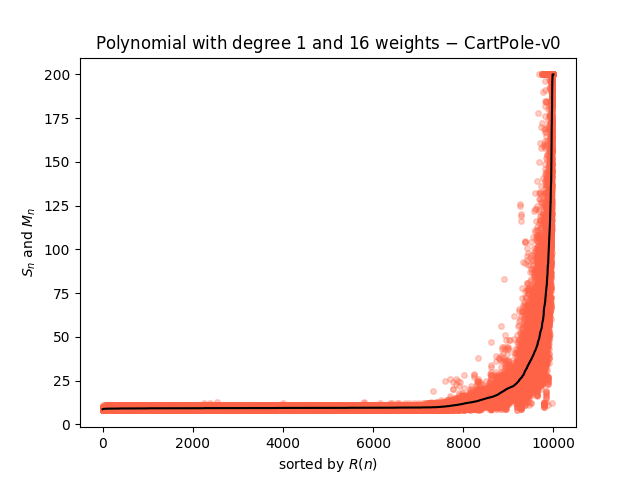
\includegraphics[width=.3\linewidth]{experiment_1/with_bias/PolynomialNN_degree_1_scatter_score.png}
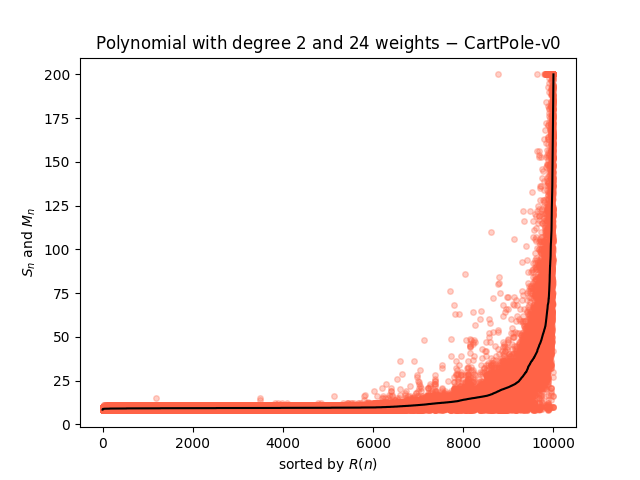
\includegraphics[width=.3\linewidth]{experiment_1/with_bias/PolynomialNN_degree_2_scatter_score.png}
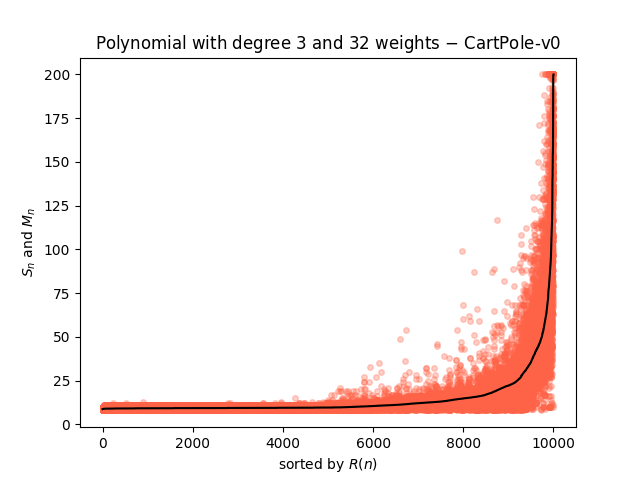
\includegraphics[width=.3\linewidth]{experiment_1/with_bias/PolynomialNN_degree_3_scatter_score.png}}
\item \label{row:P1_without_bias}  \raisebox{-0.5\height}{
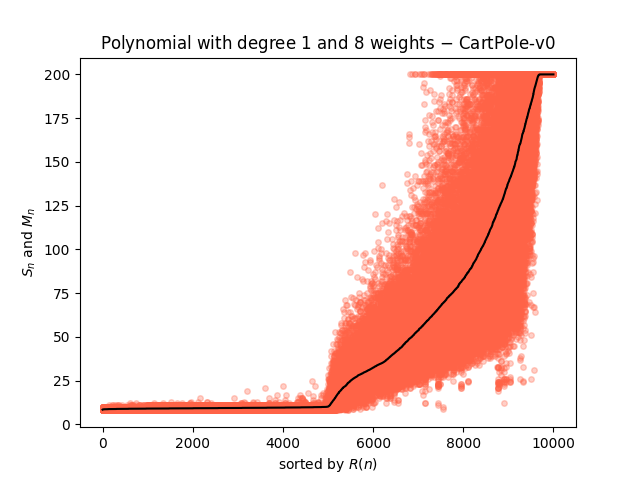
\includegraphics[width=.3\linewidth]{experiment_1/without_bias/PolynomialNN_degree_1_scatter_score.png}
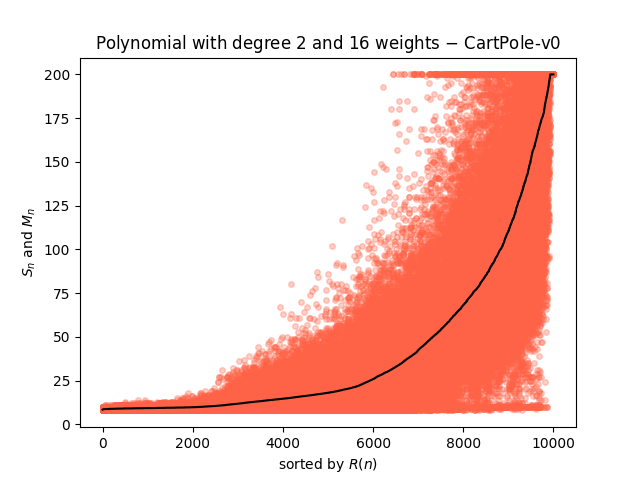
\includegraphics[width=.3\linewidth]{experiment_1/without_bias/PolynomialNN_degree_2_scatter_score.png}
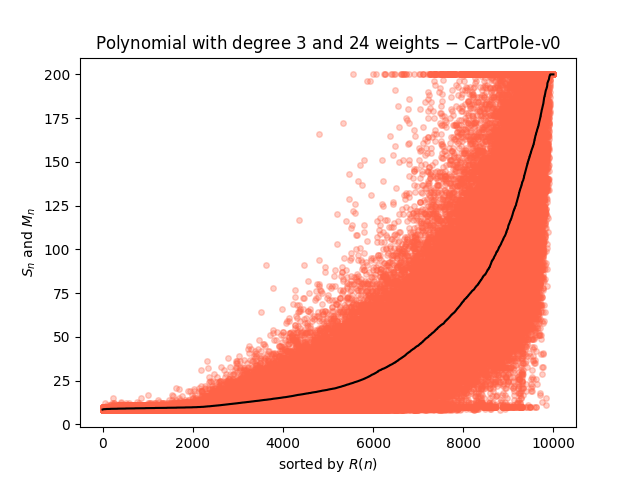
\includegraphics[width=.3\linewidth]{experiment_1/without_bias/PolynomialNN_degree_3_scatter_score.png}}
\end{figrow}
\vspace*{-5mm}
\caption{Results of $P_1$ with bias (a) and without bias (b)}
\label{fig:results_p1}
\end{subfigure}
\begin{subfigure}{\textwidth}
\begin{figrow}
\item \label{row:P2_with_bias} \raisebox{-0.5\height}{
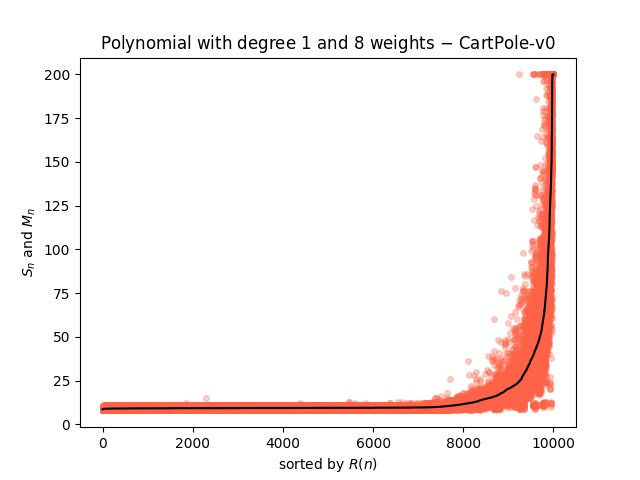
\includegraphics[width=.3\linewidth]{experiment_1/with_bias/Polynomial_degree_1_scatter_score.png}
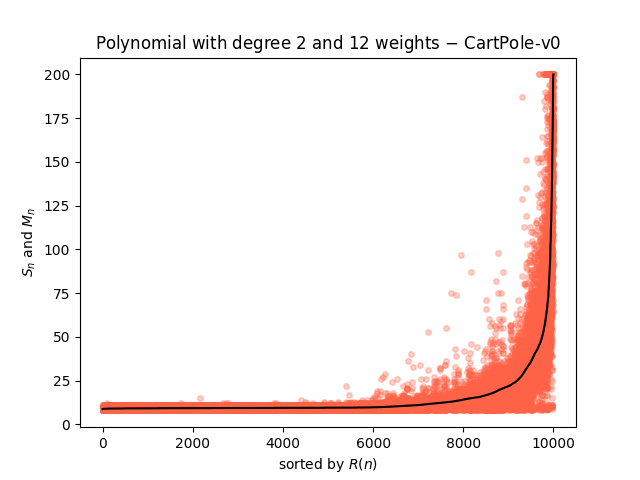
\includegraphics[width=.3\linewidth]{experiment_1/with_bias/Polynomial_degree_2_scatter_score.png}
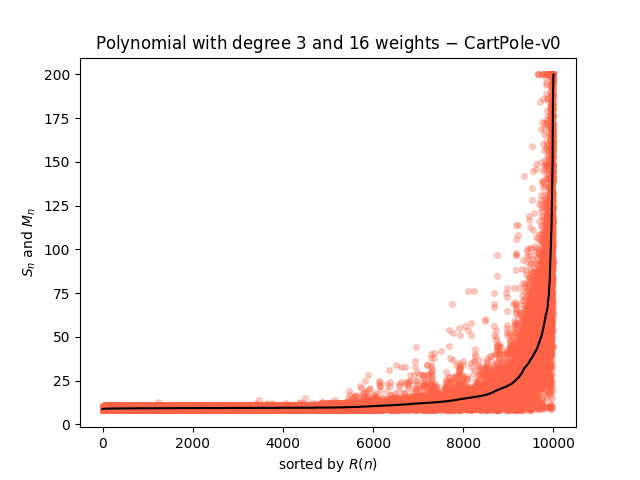
\includegraphics[width=.3\linewidth]{experiment_1/with_bias/Polynomial_degree_3_scatter_score.png}}
\item \label{row:P2_without_bias}  \raisebox{-0.5\height}{
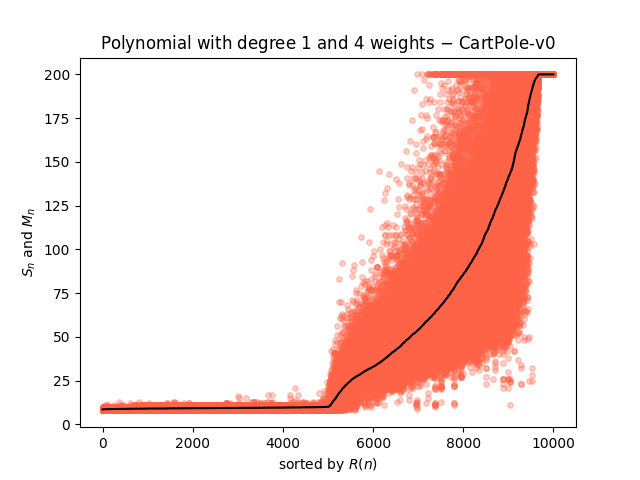
\includegraphics[width=.3\linewidth]{experiment_1/without_bias/Polynomial_degree_1_scatter_score.png}
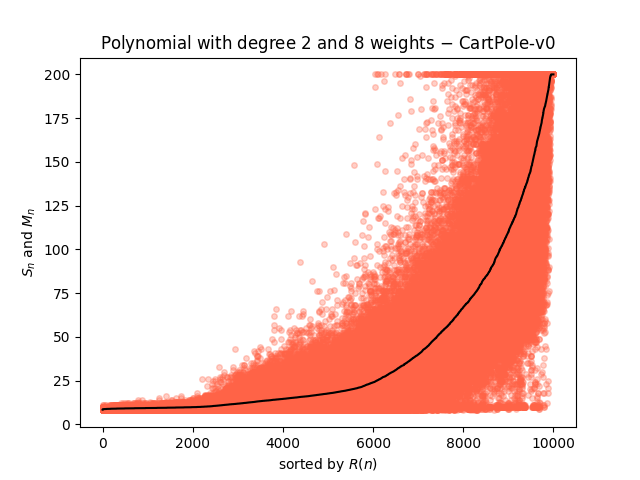
\includegraphics[width=.3\linewidth]{experiment_1/without_bias/Polynomial_degree_2_scatter_score.png}
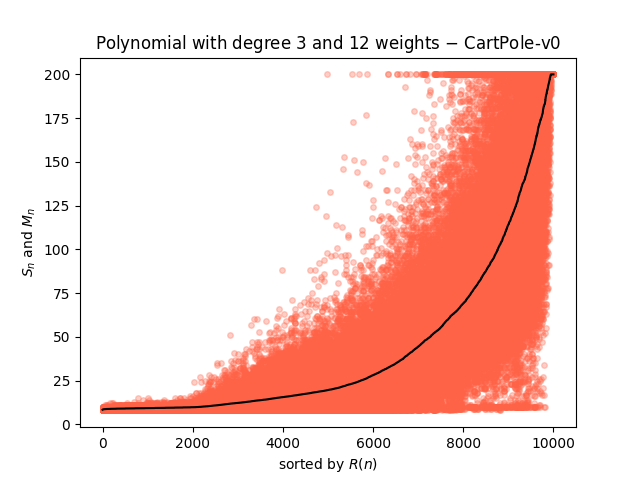
\includegraphics[width=.3\linewidth]{experiment_1/without_bias/Polynomial_degree_3_scatter_score.png}}
\end{figrow}
\vspace*{-5mm}
\caption{Results of $P_2$ with bias (a) and without bias (b)}
\label{fig:results_p2}
\end{subfigure}
\caption[Results of experiment 1: polynomial models]{
  \textbf{Results of experiment 1: polynomial models.}
   The figures show the results of the first experiment with the two polynomial models. On the $x-$axis, we have the rank of each sample. On the $y-$axis, we have the scores of all samples and the mean as a lineplot. Each subplot shows the performance of the model with bias in row (a) and without bias in row (b). As we can see, both models perform equally good or bad. However, there is a huge difference in performance whether we are working with or without bias. In addition, we can see a difference in the slope of the mean values between polynomials with degree 1 and one with a higher degree.
}
\label{fig:experiment_1_polynomial}
\end{figure}
As we can see in the images, the plots of the two models almost look identical. Both models performed equally good or bad despite their different architecture and the different number of weights. Because of this similarity, I will not go into each model independently but instead discuss further results for both of them.

Looking at the linear model without bias, we can see a striking resemblance to the performance of the neural network previously shown in Section~\ref{ssec:benchmarks}. Looking further at the linear model, we can see that the curve of the mean score stays low until around $5'000$ but then goes up relatively steeply. That means that the linear model fails around 50\% miserably. However, after that, we have a high probability to achieve a good score or even solve the task entirely during multiple episodes. There are also quite a few samples that could solve the task each time, indicated by the short straight black line at the top of the plot. Looking at the polynomials with degree 2, we can see that the scores increase already at around $2'000$, but the slope is less steep than for the linear model. In addition, there are fewer samples that could solve the task for each episode than there are for the linear model. Furthermore, the variance is higher for the polynomials with a higher degree compared to the linear model. If we look at the results of the polynomials with degree three, we can see that there is only a small boost compared to the polynomials of degree 2. The scores are overall slightly higher, but the slope is very similar to before. There is only a little difference between the two models even though the weights are doubled for $P_1$ and a half more for $P_2$. The large difference lies between the polynomials with degree 1 and polynomials with degree 2, respectively, degree 3. It seems that the complexity of the model depends more on the architecture of the model than on the number of weights.

In conclusion, with the linear model, we have a $50 \%$ chance of failing but the probability of actually solving the task for all episodes is higher than for the polynomials with a higher degree. That means that with the linear model, we have a larger fraction of samples that can solve the environment independent of the initialization conditions. At first glance, we could assume that this is an important aspect for such a model and choose the polynomial with degree 1 over one with a higher degree. However, we should remind ourselves that these experiments are rather unusual for an application since there is no learning involved and the number of samples is huge. In a common application, we would use some kind of training and want the model to sequentially improve its performance. Considering this aspect, when using a learning algorithm, we would not prefer the polynomials with degree 1 as we might get stuck in a fitness plateau when the algorithm has no method of dealing with this behavior.

Another observation we can make from Figure~\ref{fig:experiment_1_polynomial} is that the bias influences the performance of the model significantly. We already saw this behavior with the neural network in Section~\ref{ssec:benchmarks}. Thus, the influence of the bias is not specific to neural networks but seems to be more of a general factor.

\todo[inline]{Change title of plots: , instead of with, $P_1 / P_2$ instead of Polynomial \\ Explain fitness plateau further}

\subsection{Experiment 2}
weights / layers / neurons \\ \\
Figure~\ref{fig:experiment_2_weights} shows the results of doubling the number of weights in Subfigure~\ref{fig:NN_wfactor_2} and the results of tripling the number of weights in Subfigure~\ref{fig:NN_wfactor_3} for each network architecture. Row (a) shows the results using bias, row (b) shows the results without bias. We can barely see any difference between Subfigure~\ref{fig:NN_wfactor_2} and Subfigure~\ref{fig:NN_wfactor_3} despite the large difference in the number of weights used. Thus, we can conclude that increasing the number of weights does not impact the achieved score of the model significantly. Additionally, I conducted the same experiment with the polynomial models $P_1$ and $P_2$. We can make the same observation with these models. Therefore, changing the number of weights changes very little in the result.
\begin{figure}[!ht]
\begin{subfigure}{\textwidth}
\begin{figrow}
\item \label{row:NN_with_bias_wfactor_2} \raisebox{-0.5\height}{
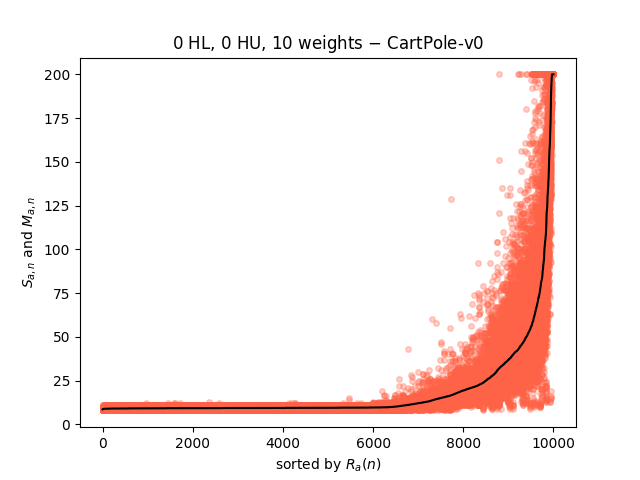
\includegraphics[width=.3\linewidth]{experiment_2/weights/weight_factor_2/with_bias/HL_0_HU_0_scatter_score.png}
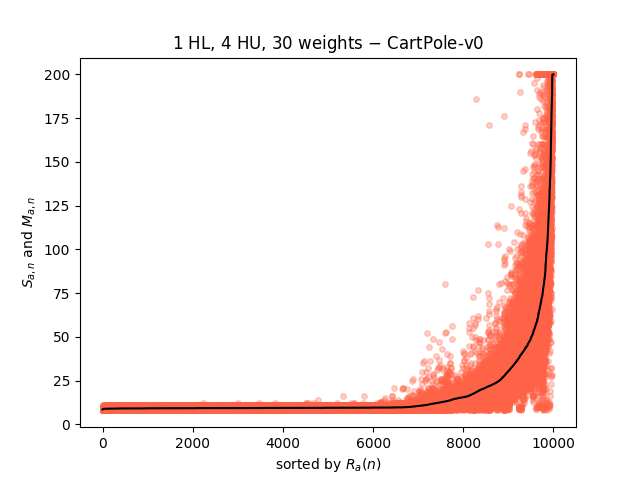
\includegraphics[width=.3\linewidth]{experiment_2/weights/weight_factor_2/with_bias/HL_1_HU_4_scatter_score.png}
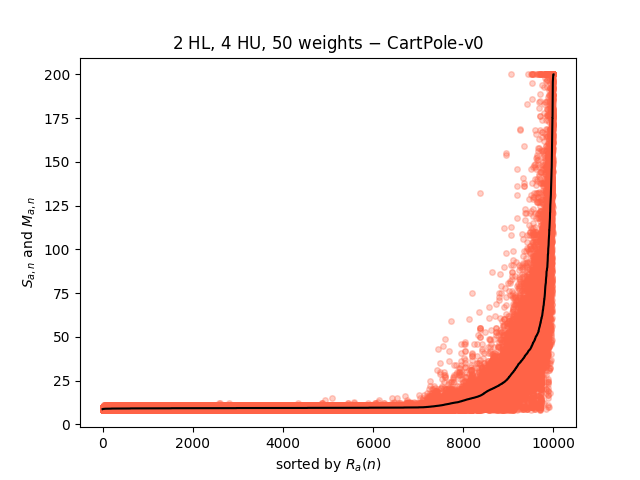
\includegraphics[width=.3\linewidth]{experiment_2/weights/weight_factor_2/with_bias/HL_2_HU_4_scatter_score.png}}
\item \label{row:NN_without_bias_wfactor_2}  \raisebox{-0.5\height}{
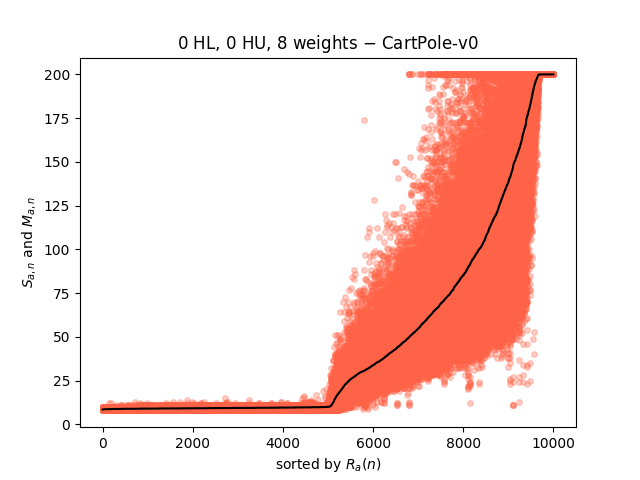
\includegraphics[width=.3\linewidth]{experiment_2/weights/weight_factor_2/without_bias/HL_0_HU_0_scatter_score.png}
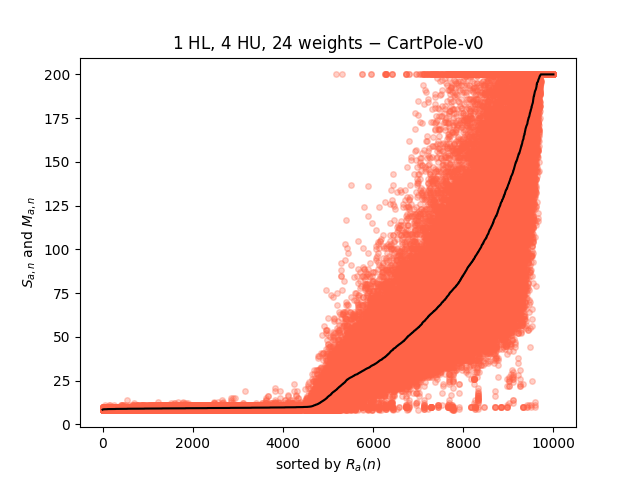
\includegraphics[width=.3\linewidth]{experiment_2/weights/weight_factor_2/without_bias/HL_1_HU_4_scatter_score.png}
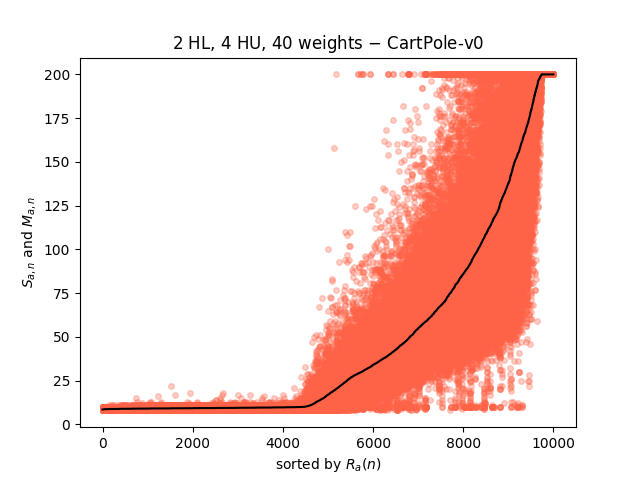
\includegraphics[width=.3\linewidth]{experiment_2/weights/weight_factor_2/without_bias/HL_2_HU_4_scatter_score.png}}
\end{figrow}
\vspace*{-5mm}
\caption{Results of doubling weights for three neural network architectures with bias (a) and without bias (b)}
\label{fig:NN_wfactor_2}
\end{subfigure}
\begin{subfigure}{\textwidth}
\begin{figrow}
\item \label{row:NN_with_bias_wfactor_3} \raisebox{-0.5\height}{
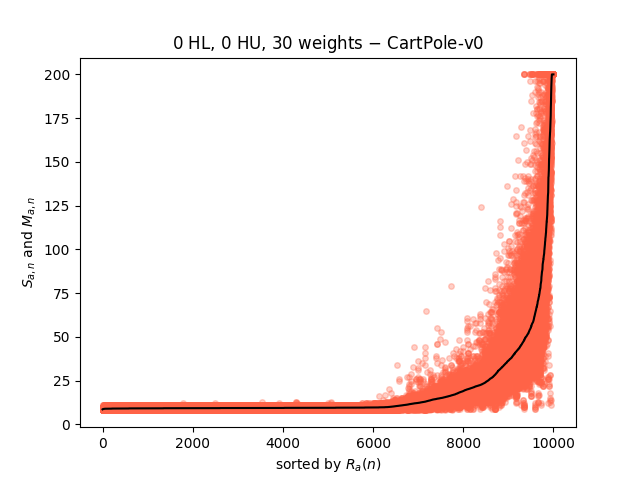
\includegraphics[width=.3\linewidth]{experiment_2/weights/weight_factor_3/with_bias/HL_0_HU_0_scatter_score.png}
\includegraphics[width=.3\linewidth]{experiment_2/weights/weight_factor_3/with_bias/HL_1_HU_4_scatter_score.png}
\includegraphics[width=.3\linewidth]{experiment_2/weights/weight_factor_3/with_bias/HL_2_HU_4_scatter_score.png}}
\item \label{row:NN_without_bias_wfactor_3}  \raisebox{-0.5\height}{
\includegraphics[width=.3\linewidth]{experiment_2/weights/weight_factor_3/without_bias/HL_0_HU_0_scatter_score.png}
\includegraphics[width=.3\linewidth]{experiment_2/weights/weight_factor_3/without_bias/HL_1_HU_4_scatter_score.png}
\includegraphics[width=.3\linewidth]{experiment_2/weights/weight_factor_3/without_bias/HL_2_HU_4_scatter_score.png}}
\end{figrow}
\vspace*{-5mm}
\caption{Results of tripling weights for three neural network architectures with bias (a) and without bias (b)}
\label{fig:NN_wfactor_3}
\end{subfigure}
\caption[Results of experiment 2: weights]{
  \textbf{Results of experiment 2: weights.}
   The figure shows the results of doubling the number of weights in Subfigure~\ref{fig:NN_wfactor_2} and the results of tripling the number of weights in Subfigure~\ref{fig:NN_wfactor_3}. Row (a) shows the results with using bias, row (b) shows the results without using bias. We can barely see any difference between Subfigure~\ref{fig:NN_wfactor_2} and Subfigure~\ref{fig:NN_wfactor_3} despite the largely different number of weights used.
}
\label{fig:experiment_2_weights}
\end{figure}

Figure~\ref{fig:experiment_2_layers} shows the results of altering the number of layers in a network.
\begin{figure}[!ht]
\begin{figrow}
\item \label{row:NN_with_bias_layers} \raisebox{-0.5\height}{
\includegraphics[width=.3\linewidth]{experiment_2/layers/with_bias/HL_4_scatter_score.png}
\includegraphics[width=.3\linewidth]{experiment_2/layers/with_bias/HL_6_scatter_score.png}
\includegraphics[width=.3\linewidth]{experiment_2/layers/with_bias/HL_8_scatter_score.png}}
\item \label{row:NN_without_layers}  \raisebox{-0.5\height}{
\includegraphics[width=.3\linewidth]{experiment_2/layers/without_bias/HL_4_scatter_score.png}
\includegraphics[width=.3\linewidth]{experiment_2/layers/without_bias/HL_6_scatter_score.png}
\includegraphics[width=.3\linewidth]{experiment_2/layers/without_bias/HL_8_scatter_score.png}}
\end{figrow}
\caption[Results of experiment 2: layers]{
  \textbf{Results of experiment 2: layers.}
   .
}
\label{fig:experiment_2_layers}
\end{figure}

\begin{figure}[!ht]
\begin{figrow}
\item \label{row:NN_with_bias_neurons} \raisebox{-0.5\height}{
\includegraphics[width=.3\linewidth]{experiment_2/neurons/with_bias/HL_2_HU_5_scatter_score.png}
\includegraphics[width=.3\linewidth]{experiment_2/neurons/with_bias/HL_2_HU_8_scatter_score.png}
\includegraphics[width=.3\linewidth]{experiment_2/neurons/with_bias/HL_2_HU_10_scatter_score.png}}
\item \label{row:NN_without_neurons}  \raisebox{-0.5\height}{
\includegraphics[width=.3\linewidth]{experiment_2/neurons/without_bias/HL_2_HU_5_scatter_score.png}
\includegraphics[width=.3\linewidth]{experiment_2/neurons/without_bias/HL_2_HU_8_scatter_score.png}
\includegraphics[width=.3\linewidth]{experiment_2/neurons/without_bias/HL_2_HU_10_scatter_score.png}}
\end{figrow}
\caption[Results of experiment 2: neurons]{
  \textbf{Results of experiment 2: neurons.}
   .
}
\label{fig:experiment_2_neurons}
\end{figure}

% !TEX root = ../main.tex

\chapter{Conclusion}
\label{ch:conclusions}

This work's driving question was whether we could find alternative models for reinforcement problems whose performance is comparable to the commonly used neural network model. To investigate how these models compare to neural networks and what advantages they have, two research questions were introduced in Section~\ref{sec:research_questions}. In addition, one research question was formulated concerning the architecture of a model for additional analysis.

\paragraph*{RQ1: How do function approximators other than neural networks compare with the latter?} In this work, I directly compared the alternative models, the polynomial and binary tree models, to neural networks. The polynomial model produced results comparable to those of neural networks. For the environment \verb|CartPole|, it delivered a more desirable score distribution for polynomials of degrees two and three. However, we would still prefer neural networks to tackle the problem of the \verb|Acrobot| environment. The environment \verb|MountainCar| seems to produce the same score distribution regardless of the model used. Thus, we cannot conclude that using the polynomial model robustly produces better results or results comparable to neural networks.

On the other hand, the binary tree model could deliver comparable results and even outperformed neural networks several times. The simplicity of the model did not limit the model's performance. The opposite is the case. It significantly outperformed neural networks for the environment \verb|CartPole|. Since \verb|CartPole| represents a relatively simple problem, the simple structure of binary trees is advantageous compared to the complex architecture of neural networks. Neural networks have proven that they are capable of solving many challenging problems. However, finding a good strategy with neural networks seems less efficient for a more straightforward task. The search space of the model can explain these results. A more complex model like neural networks with multiple hidden layers has a much larger search space in which they search for a good strategy for a given task. A large search space is a disadvantage when the task is easier to solve. Thus, we must carefully select our approach and adapt to the complexity of the task we want to solve.

The environment \verb|MountainCar| again produces a similar score distribution. The mean values seem to be identical. There are, however, a few higher individual scores for the binary tree model. As we can see in the results, the problem implemented in \verb|MountainCar| is hard to solve by RWG. All of the tested models showed similar findings. The large fitness plateau remains for all of them. To solve the problem, we need a learning algorithm high in exploration. For this use case, techniques in black-box optimization offer a good framework. Training a model with a learning algorithm prone to getting stuck in a local optimum will likely not result in a robust model that can solve the task. Also for the environment \verb|Acrobot|, the results of the two models look very similar. Although there are a few differences, both models seem equally suited to solve this task with the proper learning technique. Since a fitness plateau is present, an explorative learning algorithm should produce the best results.

Although the binary tree model only outputs discrete actions that are fixed, the results for the environment \verb|Pendulum| can compare to those of neural networks. Again, both models seem to be suited to solve the task reliably with an appropriate learning algorithm. In this case, the danger of being stuck in a local optimum is less prevalent than for the environment \verb|Acrobot|. Thus, the learning algorithm does not have to be as explorative. The environment \verb|MountainCarContiuous| delivered counterintuitive results. The restriction of the binary tree model to only output the two actions -1 and 1 from the otherwise continuous action space negatively influenced the model's performance. However, changing the actions from -1 and 1 to 0 and 1 resulted in a significantly better score distribution. Since the action defines the directional force applied to the car, a value between 0 and 1 means that we apply no force at all or actively push the car to the right in the direction of the target. Thus, the results show that the model does not necessarily have to learn to accelerate the car to the left and right to solve the task.

To conclude these findings, the binary tree model looks promising for problems in reinforcement learning. Combined with a suited learning technique, it should robustly produce results comparable to those of neural networks.

\paragraph*{RQ2: What advantages and disadvantages can we see with other function approximators?} With neural networks, we have many hyperparameters that need fine-tuning. We can completely change the model architecture by changing the number of layers or the number of neurons. We have to set many other components, like the activation function. In both the polynomial model and the binary tree model, we have only one parameter, namely the degree of the polynomial and the number of nodes of the binary tree. Thus, finding a suitable configuration of the architecture of the alternative is straightforward and does not need much effort as opposed to neural network models. In addition, the binary tree model offers much more insight into decision-making than the neural network model. To comprehend how a neural network makes a decision is very hard. The binary tree model offers much more interpretability in that sense.

\paragraph{RQ3: How does the bias influence the performance of the model?} Adding bias had a negative impact on all discrete models for the polynomial model and on almost all five classic control environments for the neural network model. In my experiments with the number of weights, the number of layers, and the number of neurons, none of these changes influenced the model's performance as much as the bias did. There seems to be something specific about the use of bias that changes the performance for these environments in the setting of RWG. Why this is the case needs further research. However, there are two exceptions. The environment \verb|MountainCarContiuous| was very reactive to each change in the architecture or the number of weights. The environment \verb|Pendulum| did not show a significant difference when using bias vs. when not using bias. A change in the architecture or the number of weights affected it similarly.


\section{Future Work}
There is much further research that can be done in this area. This work represents the first step in the direction of alternative models like the binary tree model. This thesis showed that the binary tree model looks promising and can produce results comparable to neural networks while maintaining a simple architecture and interpretability. However, it would be interesting how we can adapt the model to work better on specific problems. The current implementation of the model can undoubtedly be improved. For continuous action spaces, we can adapt the leaf nodes to be included in the learning algorithm or implement a function instead of outputting a fixed action.

So far, no practical learning technique has been involved. It would be interesting to see how the model performs with CMA-ES instead of RWG. Additionally, the model should be tested in more challenging benchmark problems like the environment \verb|BipedalWalker| also included in the set of environments provided by the OpenAI Gym interface.

Finally, it would be interesting to see how other models perform in this setting. With techniques in black-box optimization, there are numerous possibilities. For example, we could use an adapted version of the Fourier transform.


%----------------------------------------------------------------------------------------
%	BIBLIOGRAPHY
%----------------------------------------------------------------------------------------
\printbibliography[heading=bibintoc]


%----------------------------------------------------------------------------------------
%   APPENDIX
%----------------------------------------------------------------------------------------
% Rarely required, only if extra material particularly voluminous
%% !TEX root = ../main.tex

\chapter{Appendix} % Main appendix title
\label{ch:appendix}

\section{Additional Plots}
% \begin{figure}[!ht]
% \begin{figrow}
% \item \label{row:Polynomial2_CartPole}  \raisebox{-0.5\height}{
% \includegraphics[width=.3\linewidth]{experiment_1/without_bias/CartPole-v0_PolynomialNN_degree_1_scatter_score}
% \includegraphics[width=.3\linewidth]{experiment_1/without_bias/CartPole-v0_PolynomialNN_degree_2_scatter_score}
% \includegraphics[width=.3\linewidth]{experiment_1/without_bias/CartPole-v0_PolynomialNN_degree_3_scatter_score}}
% \item \label{row:Polynomial2_Acrobot}  \raisebox{-0.5\height}{
% \includegraphics[width=.3\linewidth]{experiment_1/without_bias/Acrobot-v1_PolynomialNN_degree_1_scatter_score}
% \includegraphics[width=.3\linewidth]{experiment_1/without_bias/Acrobot-v1_PolynomialNN_degree_2_scatter_score}
% \includegraphics[width=.3\linewidth]{experiment_1/without_bias/Acrobot-v1_PolynomialNN_degree_3_scatter_score}}
% \item \label{row:Polynomial2_MountainCar}  \raisebox{-0.5\height}{
% \includegraphics[width=.3\linewidth]{experiment_1/without_bias/MountainCar-v0_PolynomialNN_degree_1_scatter_score}
% \includegraphics[width=.3\linewidth]{experiment_1/without_bias/MountainCar-v0_PolynomialNN_degree_2_scatter_score}
% \includegraphics[width=.3\linewidth]{experiment_1/without_bias/MountainCar-v0_PolynomialNN_degree_3_scatter_score}}
% \end{figrow}
% \caption[Results for the classic control environments using polynomials]{
%   \textbf{Results for the discrete classic control environments using the polynomial model $\mathbf{P_1}$.}
%    Each row shows the results of one environment. The columns represent the different degrees of the polynomials. In these plots the model $P_1$ was used.
% }
% \label{fig:results_Polynomial2}
% \end{figure}
% The color of links can be changed to your liking using:
% {\small\verb!\hypersetup{urlcolor=red}!}, or
% {\small\verb!\hypersetup{citecolor=green}!}, or
% {\small\verb!\hypersetup{allcolor=blue}!}.
% \noindent If you want to completely hide the links, you can use:
% {\small\verb!\hypersetup{allcolors=.}!}, or even better:
% {\small\verb!\hypersetup{hidelinks}!}.
% \noindent If you want to have obvious links in the PDF but not the printed text, use:
% {\small\verb!\hypersetup{colorlinks=false}!}.



%----------------------------------------------------------------------------------------
\end{document}
% That's all folks
